\documentclass[12pt,a4paper]{article}
\usepackage[a4paper,top=2cm,bottom=2cm,left=3cm,right=3cm,marginparwidth=1.75cm]{geometry}
\usepackage[colorlinks=true, allcolors=blue]{hyperref}
\usepackage{amsmath}
\usepackage{enumitem}
\usepackage{setspace}
\usepackage{titlesec}
\usepackage{graphicx}
\usepackage{hyperref}
\usepackage{karnaugh-map}
\usepackage{tfrupee}
\usepackage{subcaption}
\usepackage{rotating} % Add this in your preamble
\setlength{\parskip}{1em}
\setlength{\parindent}{0em}




\begin{document}



% University and Department Heading
\begin{center}
\thispagestyle{empty}
    \textbf{\LARGE NETAJI SUBHAS UNIVERSITY OF}\\[1em]
    \textbf{\LARGE TECHNOLOGY , DELHI}\\[2em]
    
    \textbf{\Large DEPARTMENT OF ELECTRONICS  \& }\\[1em]
    \textbf{\Large COMMUNICATION}\\[2em]

    \begin{figure}
    \centering
    \vspace{5em}
    
\includegraphics[height=0.5\linewidth]{assets/nsut logo.png}
    \vspace{2em}
    \end{figure}

    \textbf{SESSION(2024-2025)}\\[0.5em]
    \textbf{ECECC402 ELECTRONICS DESIGN WORSKHOP}\\[0.5em]
    \textbf{PROJECT DOCUMENTATION REPORT}\\[4em]
    \textbf{\LARGE ``K-MAP CALCULATOR''}\\[4em]

    \textbf{Submitted By --}\\[0.5em]
    Shivam (2023UEC2581)\\
    Karan Sharma (2023UEC2600)\\
    Aadarsh Sahni (2023UEC2609)\\
\end{center}



  



\newpage
\thispagestyle{empty}
% Abstract
\begin{center}
    \textbf{\large Abstract}
\end{center}


This is the report of our 4th semester project of the Electronic Design Workshop (EDW) course. This report will give the reader an overview about the steps which were involved in the making of the K-Map Calculator. The project is about the making of K-Map Calculator that will solve the case of 4 variables. The main code to solve the K-Map was developed ourselves in C++. Firstly circuits were simulated on Wokwi (esp32 simulator) to test the outcomes. Then it was implemented on breadboard. Finally the PCB was made using a zeroboard and enclosure was designed. The results of the calculator are accurate. Calculator takes input by 16 switches. Each switch represents a K-Map cell (minterm). Each cell have 3 inputs possible: logic-1, 0 \& Don’t Care. The calculator displays the K-Map groups via LED output and the final string expression on the LCD screen.

Total combinations of inputs possible in the device is:
\[
3 \times 3 \times 3 \ldots \text{(16 times)} = 3^{16} = 4,30,46,721
\]


  \begin{center}
    \vspace{2em}
    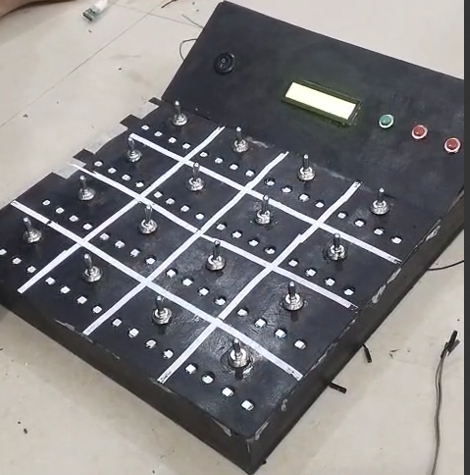
\includegraphics[height=0.75\linewidth]{assets/calc2.png}
    \vspace{2em}\\
    \textit{Final image of the calculator}
  \end{center}






\newpage
\thispagestyle{empty}
% Table of Contents
\begin{center}
    \textbf{\large TABLE OF CONTENTS}
\end{center}


\begin{enumerate}[label=\arabic*.]
    \item Introduction .................................................. 1
        \begin{enumerate}[label*=\arabic*.]
                \item K-Map 
                \item Purpose of the Project 
                \item Applications of the Project
        \end{enumerate}
    \item Guide to Use Calculator ................................. 3
        \begin{enumerate}[label*=\arabic*.]
                \item Giving Input
                \item Understanding Output
                \item Next Solution Button
        \end{enumerate}
    \item Hardware Overview ......................................... 6
           \begin{enumerate}[label*=\arabic*.]
                \item List of components used
                \item Schematics
                \item Detail on main components
                \item PCB
                \item Enclosure
        \end{enumerate}
    \item Software Overview ......................................... 16
            \begin{enumerate}[label*=\arabic*.]
                \item Custom Library to solve K-Map
                \item K-Map library header file
                \item ESP32 Code Review
        \end{enumerate}

    \item Reflection ....................................................... 19
            \begin{enumerate}[label*=\arabic*.]
                \item Problems Faced
                \item Further Improvements
                \item Conclusion
        \end{enumerate}
    \item References ...................................................... 20
        
\end{enumerate}
\vspace{2em}








\newpage
\setcounter{page}{1}
\section{Introduction}
This section will briefly discuss about the concepts of a K-map and its grouping. These concepts are necessary to understand the functioning and operating the calculator. Also the purpose and applications of the project will be discussed.

\subsection{K-Map}
Digital electronics deals with discrete-valued digital signals. In general, any electronic system based on digital logic uses binary notation (zeros and ones) to represent the states of the variables involved in it. Thus, Boolean algebraic simplification is an integral part of the design and analysis of a digital electronic system. Although Boolean algebraic laws and DeMorgan's theorems can be used to achieve the objective, the process becomes tedious and error-prone as the number of variables involved increases. This necessitates using a suitable, relatively-simple simplification technique like that of the K-map, introduced by Maurice Karnaugh in 1953.

The K-map method of solving the logical expressions is referred to as the graphical technique of simplifying Boolean expressions. K-maps are also referred to as 2D truth tables as each K-map is nothing but a different format of representing the values present in a one-dimensional truth table. K-maps basically deals with the technique of inserting the values of the output variable in cells within a rectangle or square grid according to a definite pattern. The number of cells in the K-map is determined by the number of input variables and is mathematically expressed as two raised to the power of the number of input variables, i.e., $2^n$, where the number of input variables is $n$. Thus, to simplify a logical expression with two inputs, we require a K-map with 4 ($=2^2$) cells. A four-input logical expression would lead to a 16 ($=2^4$) celled-K-map, and so on.
\vspace{1em}

\textbf{Steps to Solve Expression using K-map}
\begin{enumerate}
    \item Identify minterms in the problem.
    \item For SOP put 1’s in blocks of K-map respective to the minterms (0’s elsewhere).
    \item Make rectangular groups containing total terms in power of two like 2, 4, 8 ..(except 1) and try to cover as many elements as you can in one group.
    \item From the groups made in step 3 find the product terms and sum them up for SOP form.
\end{enumerate}

    \begin{figure}
    \centering
    \vspace{2em}
    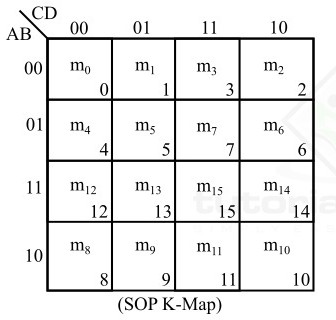
\includegraphics[height=0.5\linewidth]{assets/four-variable-k-map.jpg}
    \caption{\label{fig:frog}K-Map for 4 variables}
    \vspace{2em}
    \end{figure}


\subsection{Purpose of the Project}
To design a K-Map calculator for 4 variables which is capable of showing all possible groups, solutions and final expression. At its core this project is just a calculator which takes input from the user, perform calculations and displays the output.

\subsection{Applications of the Project}
This project can be used to solve K-map quickly. It can be used in university laboratories to help students learn about K-Map rules by practical experience.





\newpage
\section{Guide to Use the Calculator}
  \begin{figure}[h]
    \vspace{0.5em}
    \centering
    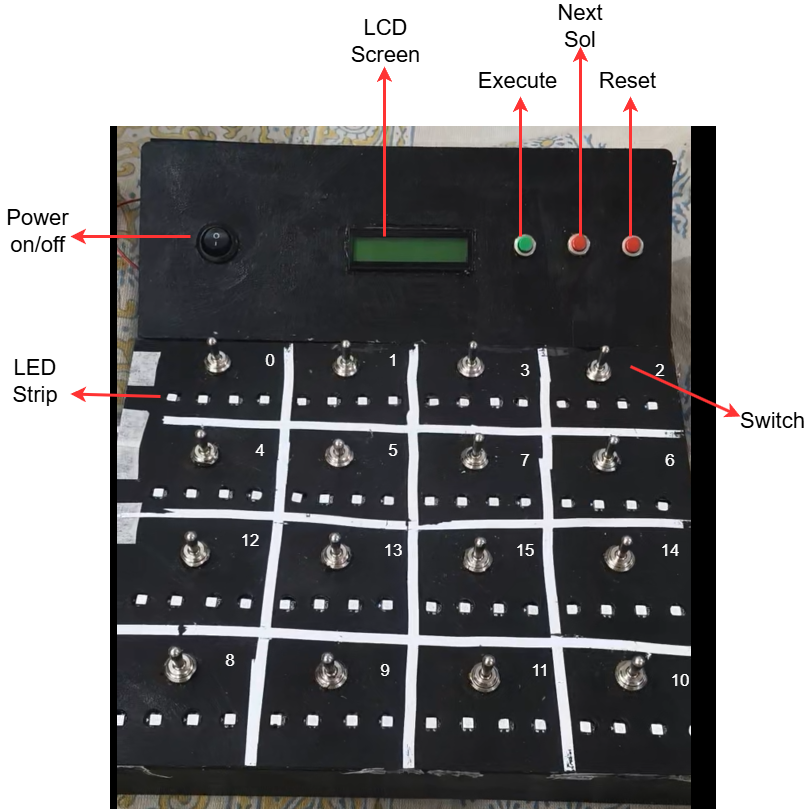
\includegraphics[height=0.75\linewidth]{assets/calc label (2).png}
    \caption{\label{fig :calc label (2)} Labeled figure showing interactive parts}
    \vspace{1em}
  \end{figure}
  
  Above figure shows  all the components accessible to the user. The calculator is powered via two 3.7V lithium ion batteries. When the power switch is turned on , the four strips light up in 4 different colors and the screen displays our names. As soon as the screen clears, the calculator is ready to take the input.

  \subsection{Giving Input}
  All the switches are in the form of K-map grid, each representing the respective minterm. Each switch can take three inputs 1,0 and Don’t care. When the switch is up it represent logic 1 at that cell. When the switch is at middle  it means logic 0. When the switch is down it means logic don’t care. The user will have to set status of each cell manually via switches for the desired solution.

\subsection{Understanding Output}
When all the switches are at desired positions, press the execute button. Wait for calculator to compute(2-3 seconds). Two forms of output will appear , first is the Boolean expression running on the screen. Second is the groupings indicated by the LEDs.\\
For example when the cells at 1,5,13 are set to logic 1 and rest to logic 0, the calculator lights up cell 1 with blue color ,cell 5 with blue \& green and cell 13 with green. All cells with same color are in same group. So in this case there are two groups \{1,5\} \& \{5,13\}. \\

\begin{figure}[h!]
  \centering
  % K-map on the left
  \begin{minipage}{0.48\textwidth}
    \centering
    % Example K-map (replace with your actual map)
    \begin{karnaugh-map}[4][4][1][$CD$][$AB$]
      \minterms{1,5,13}
      \autoterms[0]
    \implicant{1}{5}
    \implicant{5}{13}
    \end{karnaugh-map}
    \caption{K-map grouping}
  \end{minipage}
  \hfill
  % Image on the right
  \begin{minipage}{0.48\textwidth}
    \centering
    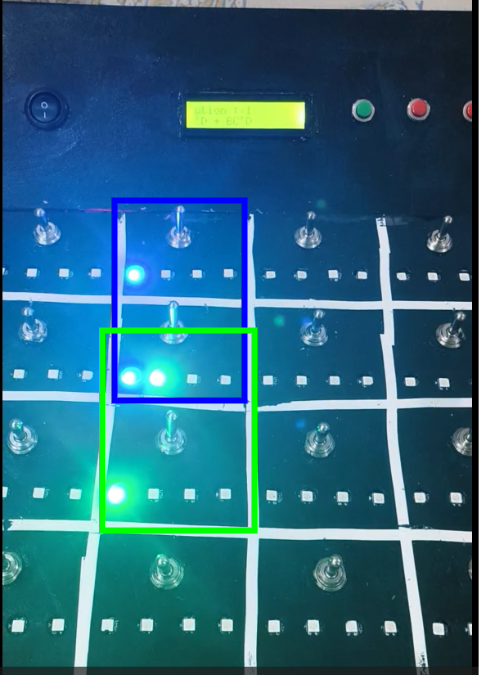
\includegraphics[width=0.7\textwidth]{assets/calc grouping.png}
    \caption{Same K-map grouping on device}
  \end{minipage}
\end{figure}

The screen will display the boolean expression corresponding to groupings. Here the group \{1,5\} corresponds to A’C’D and the group \{5,13\} corresponds to BC’D. “Solution : 1” in first line indicates that this is first solution of this input. In this case only one solution exists so same solution will appear on pressing the next solution button.

  \begin{figure}[h]
    \vspace{1em}
    \centering
    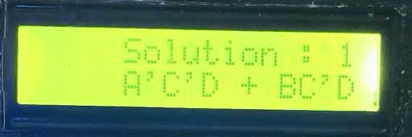
\includegraphics[width=0.5\linewidth]{assets/calc screen.png}
    \caption{\label{fig :calc label (2)} Screen Output}
    \vspace{1em}
  \end{figure}

\subsection{Next Solution Button}
For cases in which which multiple solutions can exist , next solution button will display different groupings from the previous one. When the calculator is showing the last possible solution and the next solution button is pressed, 1st solution appears again. So solutions appears in cyclic order.
\newpage

\begin{figure}[h]
    \centering
    % First image (a)
    \begin{subfigure}[t]{0.45\textwidth}
        \centering
        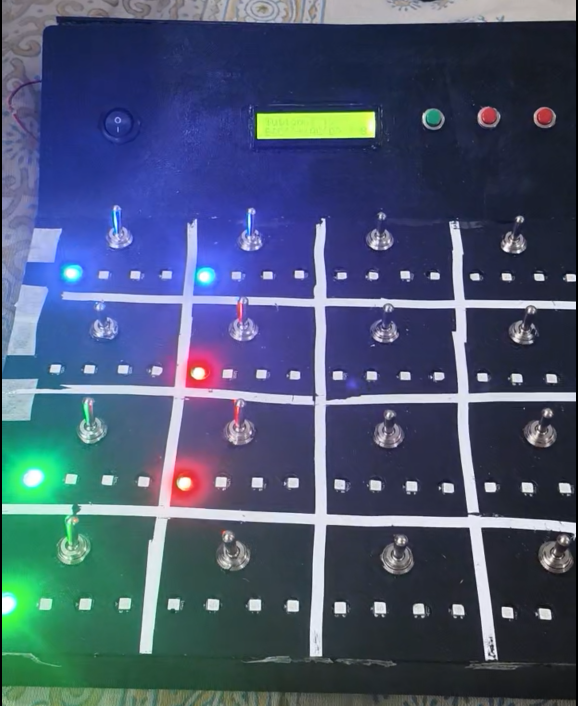
\includegraphics[width=\textwidth]{assets/sol1.png} % Replace with your image file
        \caption{}
        \label{fig:img1}
    \end{subfigure}
    \hfill
    % Second image (b)
    \begin{subfigure}[t]{0.45\textwidth}
        \centering
        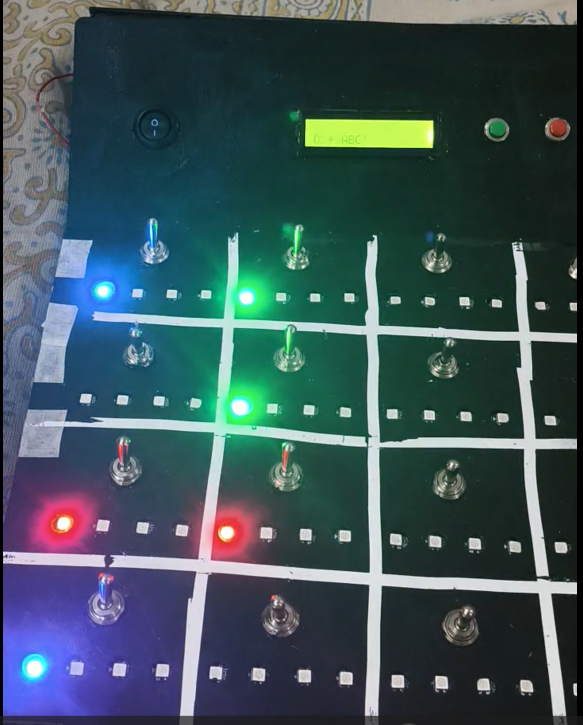
\includegraphics[width=\textwidth]{assets/sol2.png} % Replace with your image file
        \caption{}
        \label{fig:img2}
    \end{subfigure}
    % Main caption for both images
    \caption{possible groupings for same input by pressing next solution button for $\sum m(0,1,5,8,12,13)$}
    \label{fig:side-by-side}
\end{figure}


\newpage
\section{Hardware Overview}
\subsection{List of Components Used}
\begin{itemize}
  \item LCD Display(16 x 2 ) without i2c
  \item ESP32 (38 pins)
  \item CD74HC4067 (16 channel analog multiplexer)
  \item WS2812B Led Strip –  64 LEDs
\item 16 x SPDT (On-Off-On) Toggle Switch
\item 1 x SPST Switch
\item 3 x Push button 
\item 10k pot
\item 2 x 3.7V Lithium batteries
\item Buck converter(LM2596)
\item Battery Holder
\item Wires
\item Connecters
\item Header pins
\item 32 x 100k Resistors
\item 2 x 100 uF Capacitor
\item ZeroBoard
\item Acrylic Sheet
\end{itemize}


\subsection{Schematics}
The schematics were made using KiCAD software. Figure 7 focuses on connections of ESP32 with other components whereas Figure 8 focuses on supplying power to these components via the two 3.7V batteries
\begin{sidewaysfigure}
    \centering
    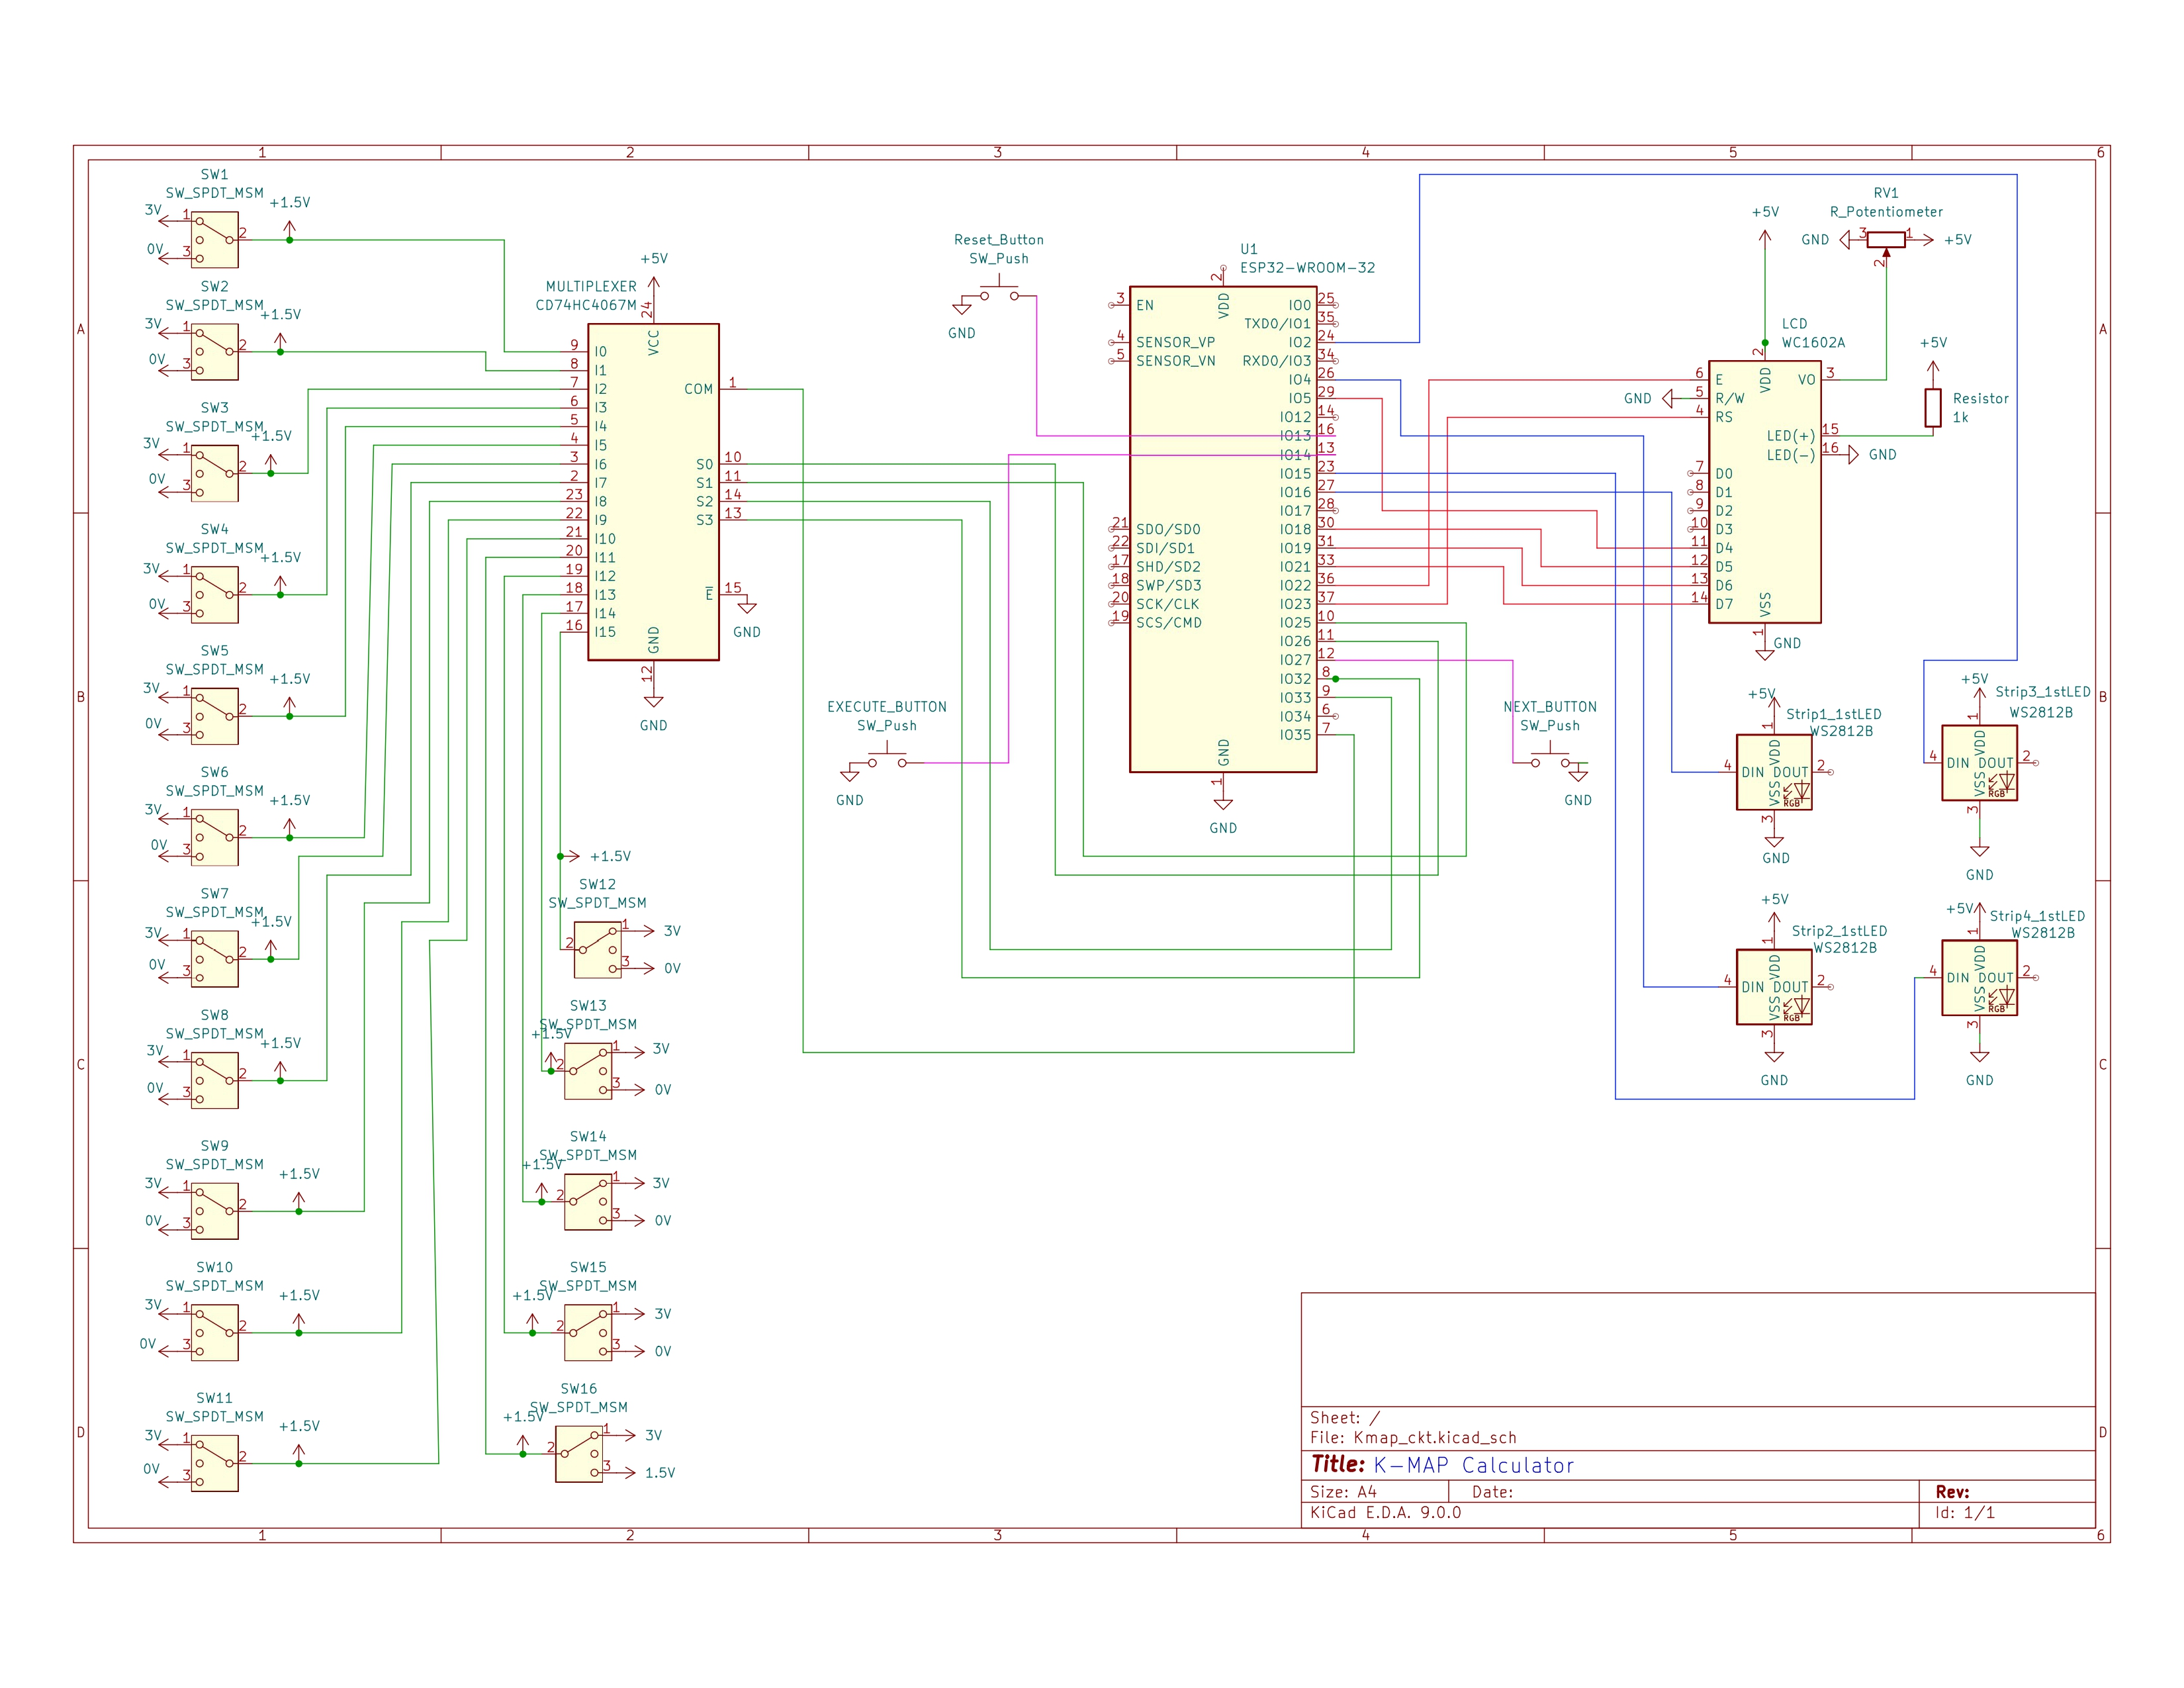
\includegraphics[width=0.9\textwidth]{assets/kmapckt.jpg}
    \caption{Schematic for connections of ESP32}
    \label{fig:yourlabel}
\end{sidewaysfigure}

\begin{sidewaysfigure}
    \centering
    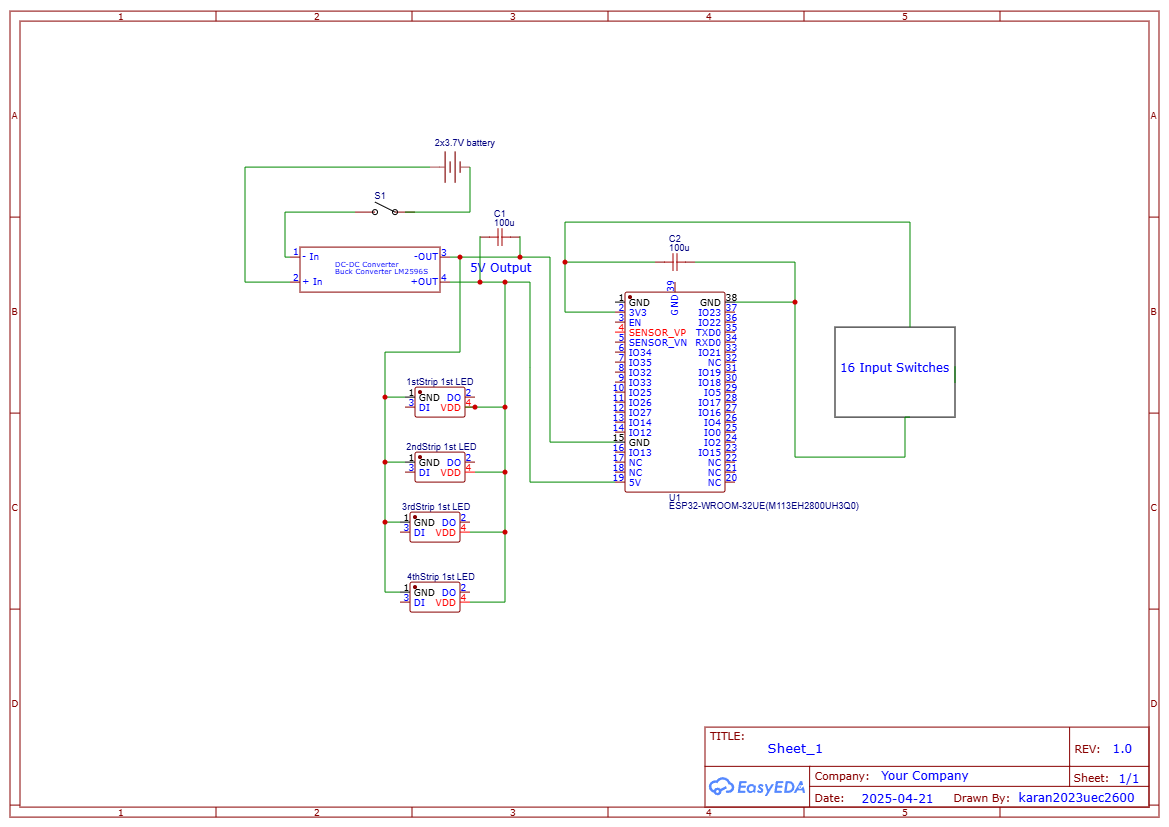
\includegraphics[width=0.9\textwidth]{assets/Schematic_final-battery_2025-04-21.png}
    \caption{Schematic for power supply to ESP32 and LEDs}
    \label{fig:yourlabel}
\end{sidewaysfigure}



\newpage
\subsection{Detail on Main Components}
\textbf{LCD Display(16 x 2 ) without i2c}\\
The term LCD stands for liquid crystal display. It is one kind of electronic
display module used in an extensive range of applications like various circuits
devices like mobile phones, calculators, computers, TV sets, etc. These dis-
plays are mainly preferred for multi-segment light-emitting diodes and seven
segments. It can be easily interfaced with microcontrollers using built in libraries
\begin{figure}[h]
    \centering
    \vspace{1em}
    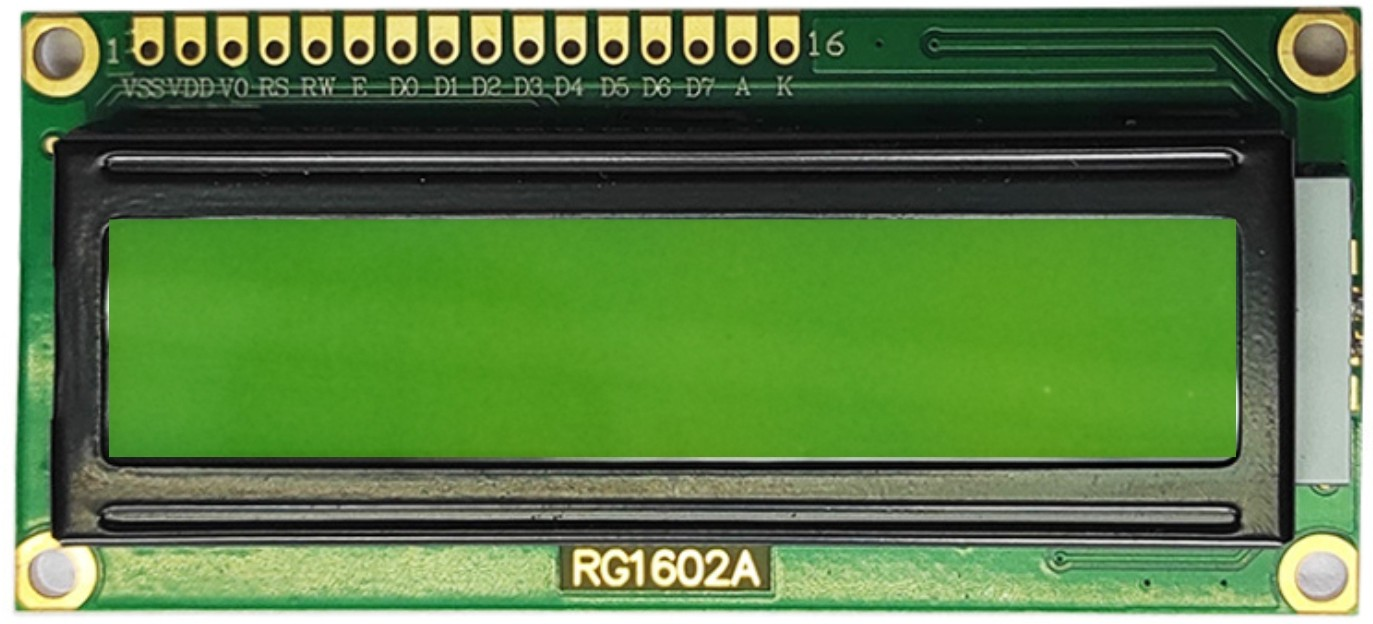
\includegraphics[width=0.5\textwidth]{assets/lcd display.jpg}
    \caption{}
    \label{fig:yourlabel}
    \vspace{1em}
\end{figure}
In this project it was used to display the Boolean expression output. The main benefits of using this module are - inexpensive; simply programmable, animations, and there are no limitations for displaying custom characters etc.

\textbf{ESP 32 (38 pins)}\\
The ESP32 38-pin variant is a popular development board based on the ESP32 series of microcontrollers from Espressif. It is widely used for IoT, smart home, and wireless communication projects due to its robust feature set and integrated wireless connectivity. It has processor Dual-core Xtensa 32-bit LX6 microprocessor, running at 160 to 240 MHz. Memory is 520 KB SRAM, 448 KB ROM. The 38-pin variant provides ample GPIOs for interfacing with sensors, actuators, and displays. Typically, up to 34 programmable GPIOs are available, though some are reserved for internal functions.
\begin{figure}[h]
    \centering
    \vspace{1em}
    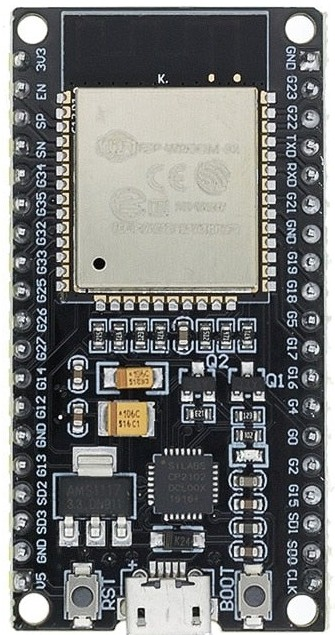
\includegraphics[height=0.3\textwidth]{assets/esp32.jpg}
    \caption{}
    \label{fig:yourlabel}

\end{figure}\\
Although no use of connectivity or wireless communication was made in our project, still it was preferred over arudino nano , due to its high number of GPIO pins, More processing power and memory and comparable price.

\textbf{CD74HC4067 (16 channel analog multiplexer)}\\
The CD74HC4067 is a high-speed CMOS 16-channel analog/digital multiplexer/demultiplexer. It is widely used for expanding the number of analog or digital I/O lines in microcontroller-based systems, allowing you to route one of 16 signals to a single pin, or vice versa. It offers 16 independent input/output channels (labeled C0–C15), selectable via four binary address pins (S0–S3). Each channel can function as either an input or output, supporting both analog and digital signals. It Operates from 2V to 6V, making it compatible with both 3.3V and 5V logic systems. The four select lines (S0–S3) determine which of the 16 channels is connected to the common I/O pin (SIG or Z). Only one channel is connected at a time.
\begin{figure}[h]
    \centering
    \vspace{1em}
    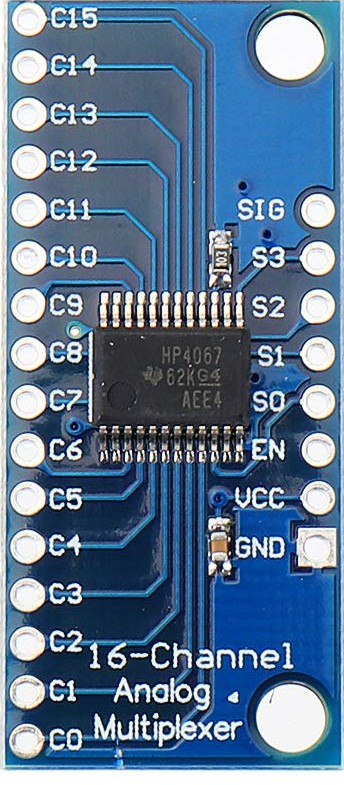
\includegraphics[height=0.3\textwidth]{assets/multiplexer.jpg}
    \caption{}
    \label{fig:yourlabel}
\end{figure}\\
This multiplexer was used to connect K-Map cell switches to each channel , then read the status of each switch one by one . If each switch was directly connected to data pins of ESP , it would lead to consumption of 16 GPIO pins. Since it is better to save pins for further expansions , this multiplexer was used

\textbf{WS2812B LED Strip}\\
WS2812b strips contain RGB LEDs, meaning each LED is actually a combination of three even tinier LEDs - one that is Red, one that is Green, and one that is Blue (hence the RGB). These are great because each color can be turned on to a different brightness level (i.e. red at full bright, green at half bright, and blue off) in order to produce millions of different colors.

\begin{figure}[htbp]
    \centering
    \begin{minipage}{0.4\textwidth}
        \centering
        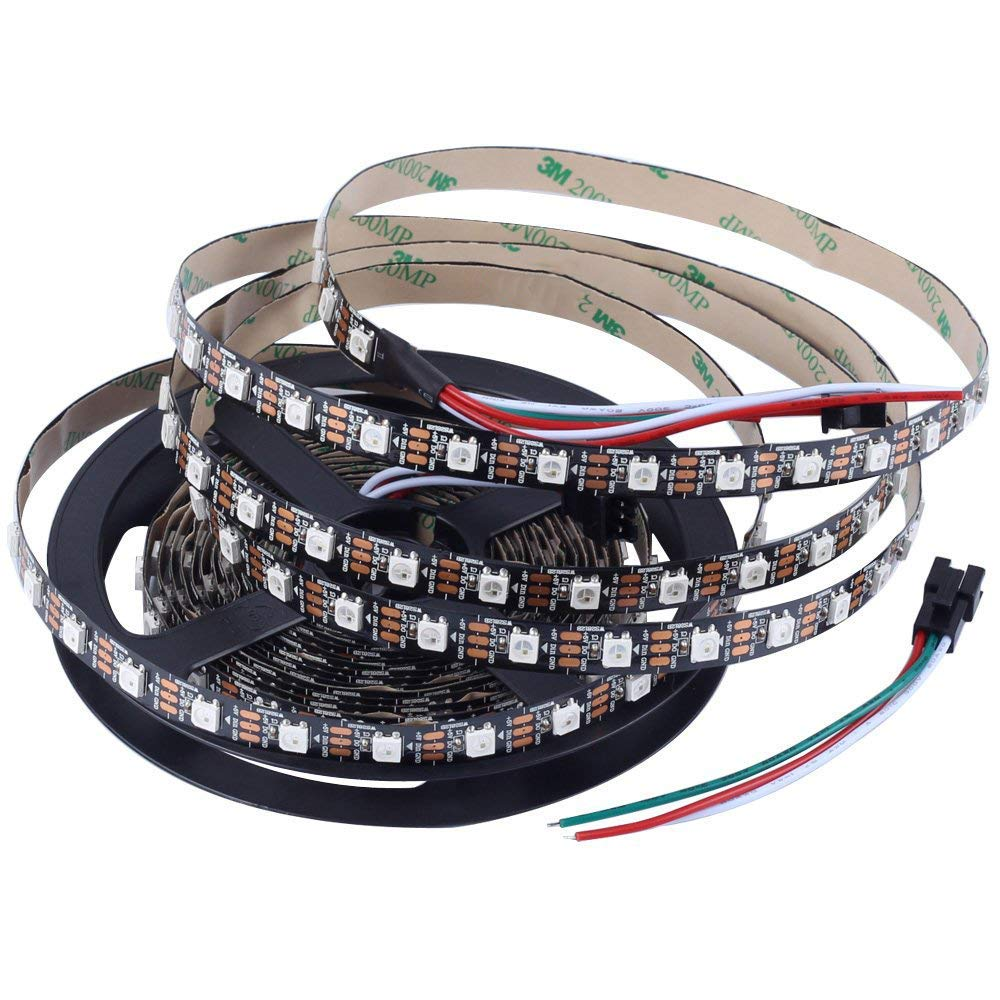
\includegraphics[width=\linewidth]{assets/led strip.jpg}
        \caption{}
        \label{fig:image1}
    \end{minipage}
    \hfill
    \begin{minipage}{0.4\textwidth}
        \centering
        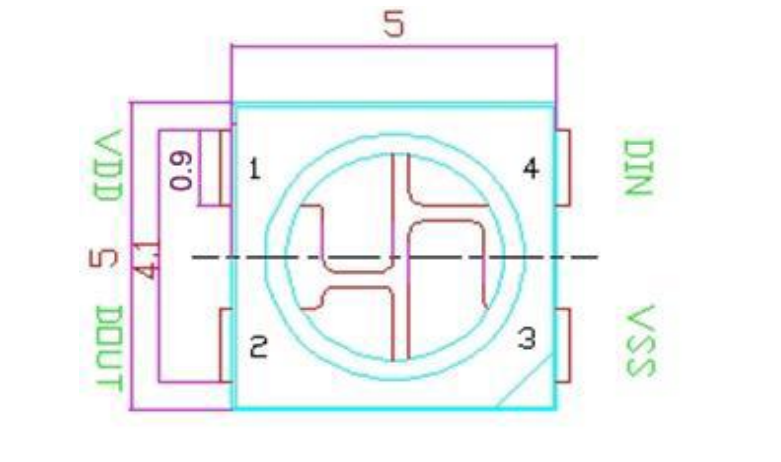
\includegraphics[width=\linewidth]{assets/indv led.png}
        \caption{Individual LED pins}
        \label{fig:image2}
    \end{minipage}
\end{figure}
The WS2812b strip has three connections, also known as pins: Power5V, Data In Din, and Ground 0V. With these three pins connected to a microcontroller, we can set the brightness and color on each individual LED in the strip. This is why it is “individually addressable” - you can control each LED independently.
This is because the  microcontroller sends more than just an 'on' or an 'off' signal to the LED strip. Instead, the Arduino uses a protocol (WS2812b) to communicate to a chip inside the first LED, which in turn communicates to the next LED down in the line, and so on. It treats the strip like an array.\\
This made the project convenient , instead of wiring each LED individually , 4 strips of 16 LED’s one for each row of K-Map was used. Each strip was connected to the data pin of ESP. Necessary logic to light up appropriate patterns were implemented in code.

\textbf{SPDT (ON-OFF-ON) Toggle Switch}\\
A SPDT (Single Pole Double Throw) 3-pin 3-way toggle switch is a versatile electrical switch commonly used for selecting between two circuits or states It has one common terminal and two output terminals, allowing the user to connect the common pin to either of the two outputs by toggling the switch
3 Positions (ON-OFF-ON): The switch can be set to one of three positions:\\
ON: Connects the common pin to one output.\\
OFF (Center): Disconnects both outputs (no connection).\\
ON: Connects the common pin to the other output\\

\begin{figure}[h]
    \centering
    \vspace{1em}
    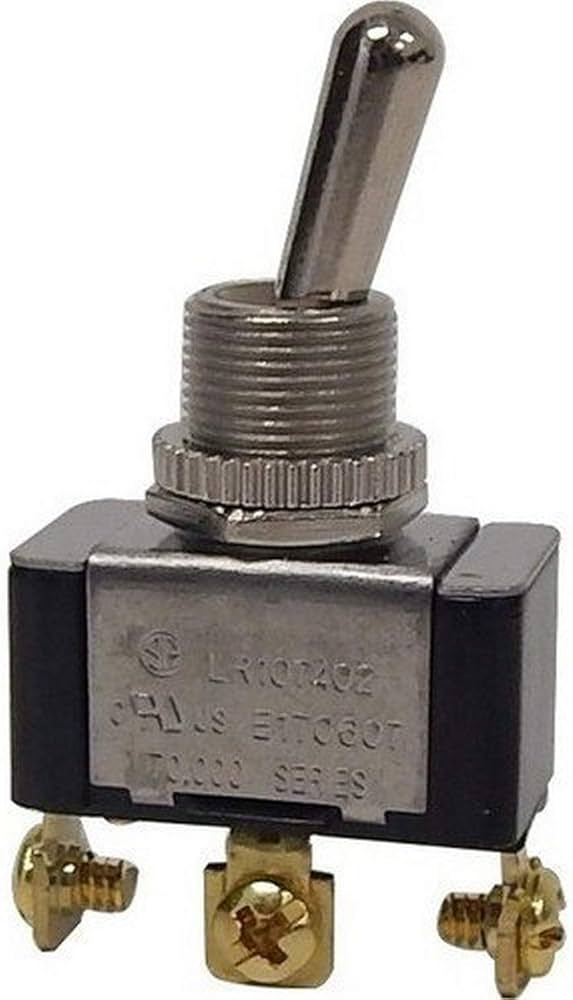
\includegraphics[height=0.3\textwidth]{assets/switch.jpg}
    \caption{}
    \label{fig:yourlabel}
\end{figure}
In our project resistors are connected between the  two ON-OFF terminals which act as voltage divider to supply different voltages to multiplexer channel at each switch position. The on terminals is supplied with 3.3V and 0V . So when the switch is in off condition the switch will send 1.5V to the channel , when the switch in ON(up) it will short the resistor and will send 3.3V to the channel. When the switch in ON(down) it shorts the other resistor and sends 0V to the channel.

\textbf{Push Button}\\
A 2-pin push button is a simple, momentary switch commonly used in electronic circuits to control the flow of current. It features two terminals that, when the button is pressed, are connected internally to complete a circuit; when released, the connection is broken. \\
\begin{figure}[h]
    \centering
    \vspace{1em}
    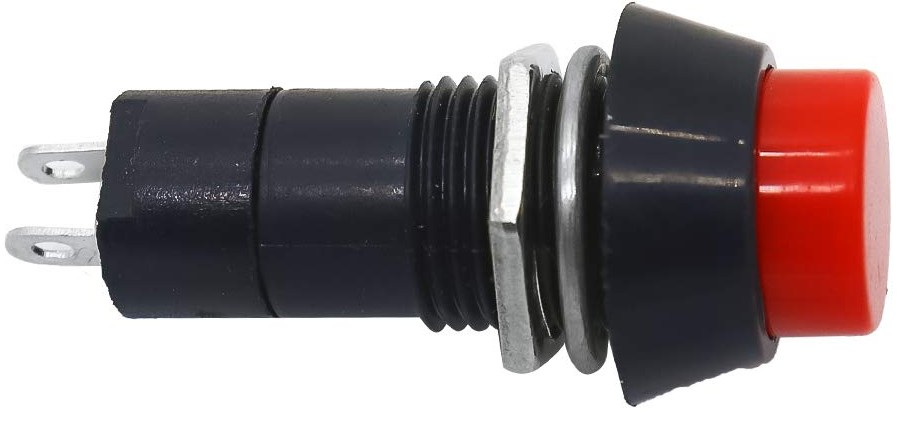
\includegraphics[width=0.2\textwidth]{assets/push button.jpg}
    \caption{}
    \label{fig:yourlabel}
\end{figure}These buttons are used as Execute, Reset and Next solution buttons. They are directly connected to 3 different GPIO pins of ESP32. When the Button is pressed 
\\ \\  \\ \\
it sends 0 to the GPIO pin otherwise it is at 1. So appropriate steps are taken after the triggering.

\textbf{SPST Switch}\\
A Single Pole Single Throw (SPST) switch is the simplest type of electrical switch, designed to control a single circuit by either opening (breaking) or closing (making) the connection. It is commonly used for basic ON/OFF control in a wide range of applications.
\begin{figure}[h]
    \centering
    \vspace{1em}
    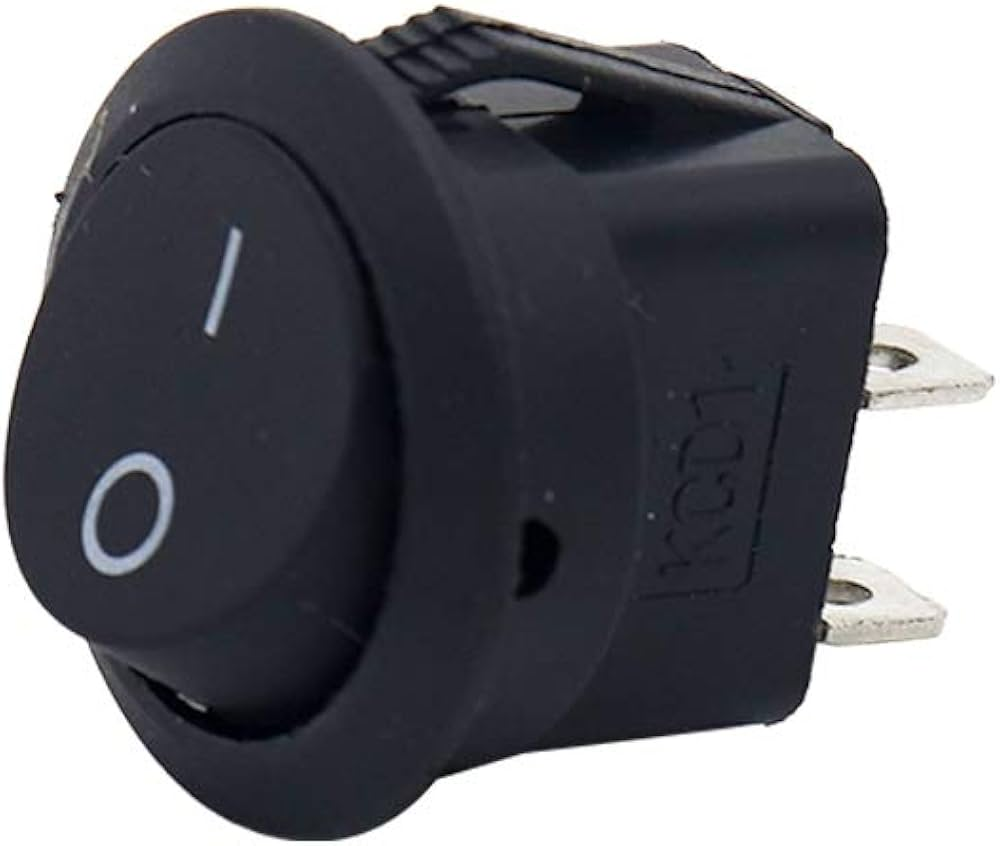
\includegraphics[width=0.2\textwidth]{assets/spst switch.jpg}
    \caption{}
    \label{fig:yourlabel}
\end{figure}
This switch was used as main On/Off switch of the calculator.\\

\textbf{3.7V Lithium battery}\\
A 3.7V lithium battery is a rechargeable power source based on lithium-ion (Li-ion) or lithium polymer (LiPo) chemistry, widely used in portable electronics and high-performance applications due to its high energy density, lightweight design, and long cycle life. Nominal Voltage: 3.7V (average voltage during discharge). Fully Charged Voltage: 4.2V (maximum voltage). Capacity is typically ranges from 500mAh to 3500mAh for single cells.
\begin{figure}[h]
    \centering
    \vspace{1em}
    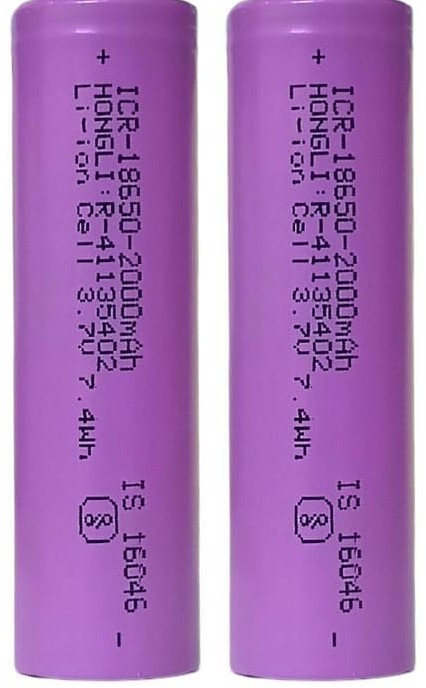
\includegraphics[width=0.2\textwidth]{assets/battery.jpg}
    \caption{}
    \label{fig:yourlabel}
\end{figure}\\
Two such batteries are used in project as main power source.
The batteries need to be physically taken out from the holder and recharged or replaced in case the calculator don’t  switch on.

\textbf{Buck converter(LM2596)}\\
The LM2596 is a popular monolithic integrated circuit designed for step-down (buck) DC-DC voltage regulation. It is widely used in power supply modules for efficiently converting higher DC voltages to lower, regulated outputs, making it ideal for battery-powered and embedded electronics projects. Input voltage: 3-40V . Output voltage: 1.5-35V(Adjustable). Output current: Rated current is 2A, maximum 3A . Conversion efficiency: 92\% (highest)
\begin{figure}[h]
    \centering
    \vspace{1em}
    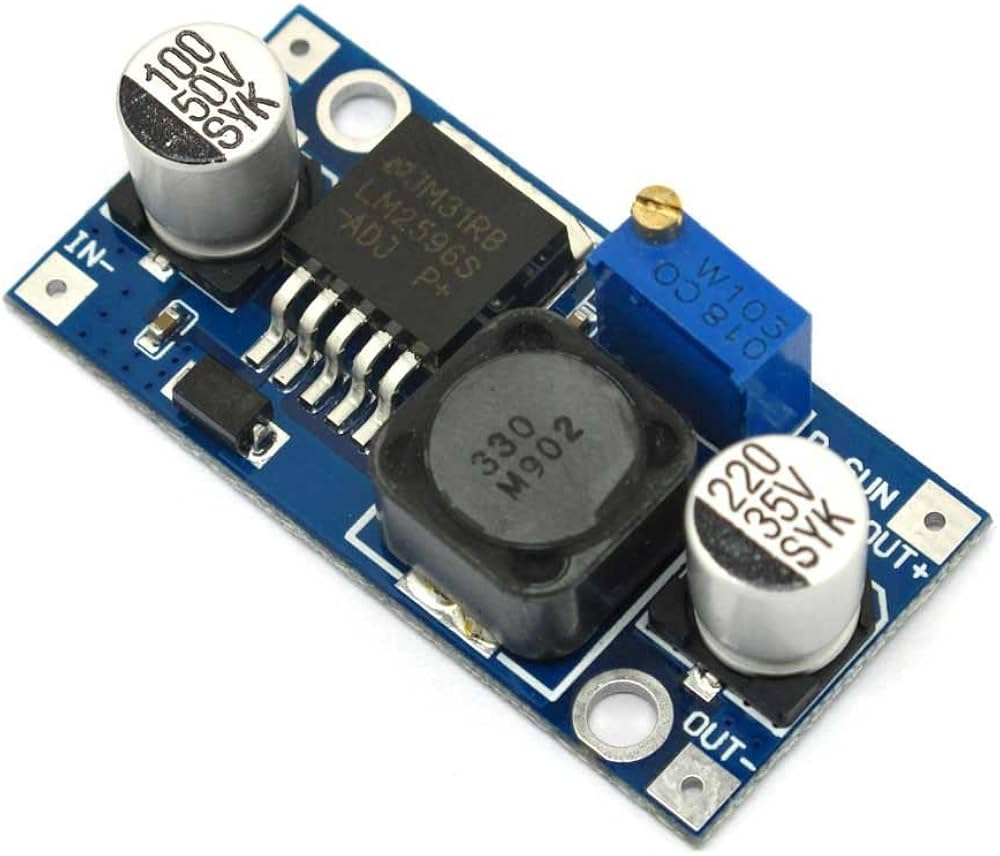
\includegraphics[width=0.4\textwidth]{assets/buck.jpg}
    \caption{}
    \label{fig:yourlabel}
\end{figure}\\
The battery is connected to the IN+ and IN- terminals, the output of the buck is adjusted by a screw to deliver constant 5V to ESP32 and LEDs.

\subsection{PCB and Wiring}
PCB was designed on a ZeroBoard. Connections were made according to the schematics. The PCB consists of ESP32 ,  CD74HC4067 sitting on header pins. Also 5V rail , 3.3V and ground rails were made. All connections were made using soldering iron. Single core wires are ideal for making PCBs and other connections as they provide flexibility and have lower risk of short circuits compared to multi-core cables.Wirings were connected to PCB using connectors. Jumper wires were connected using screw terminals.
\begin{figure}[h]
    \centering
    \vspace{1em}
    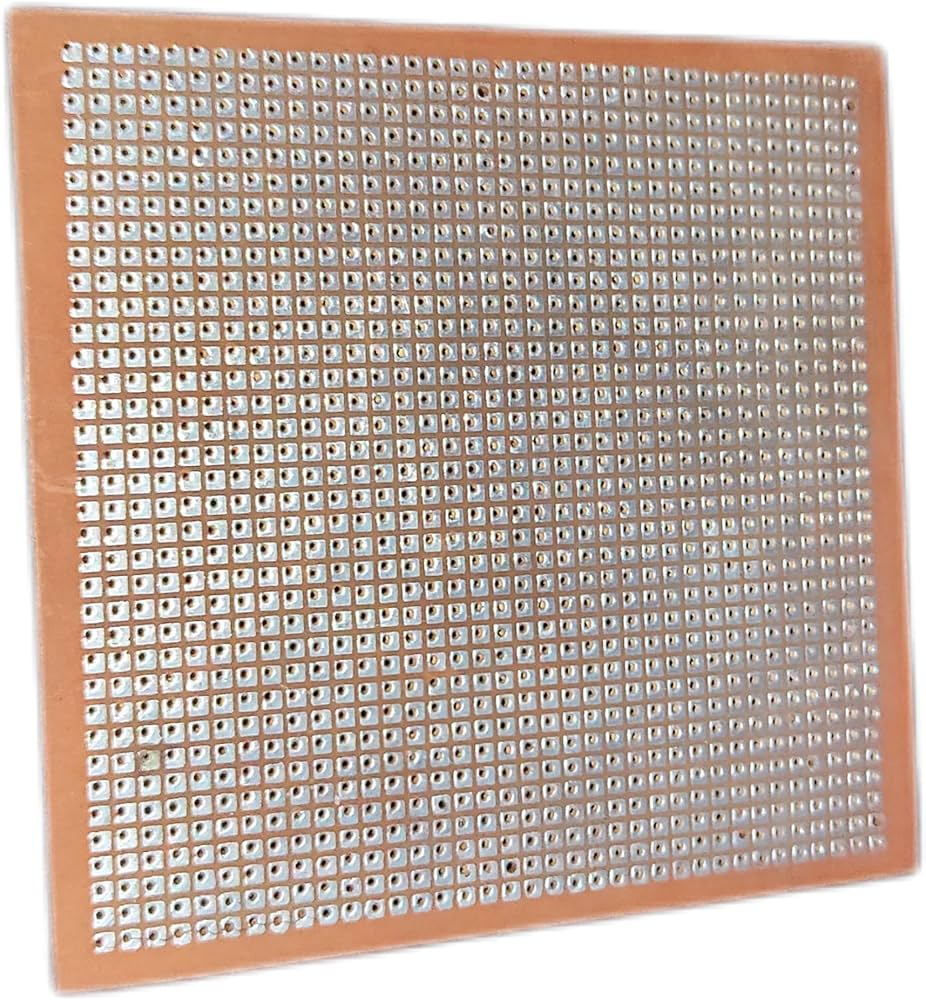
\includegraphics[width=0.3\textwidth]{assets/zeroboard.jpg}
    \caption{Blank ZeroBoard}
    \label{fig:yourlabel}
\end{figure}\\

\begin{figure}[htbp]
    \centering
    \begin{minipage}{0.47\textwidth}
        \centering
        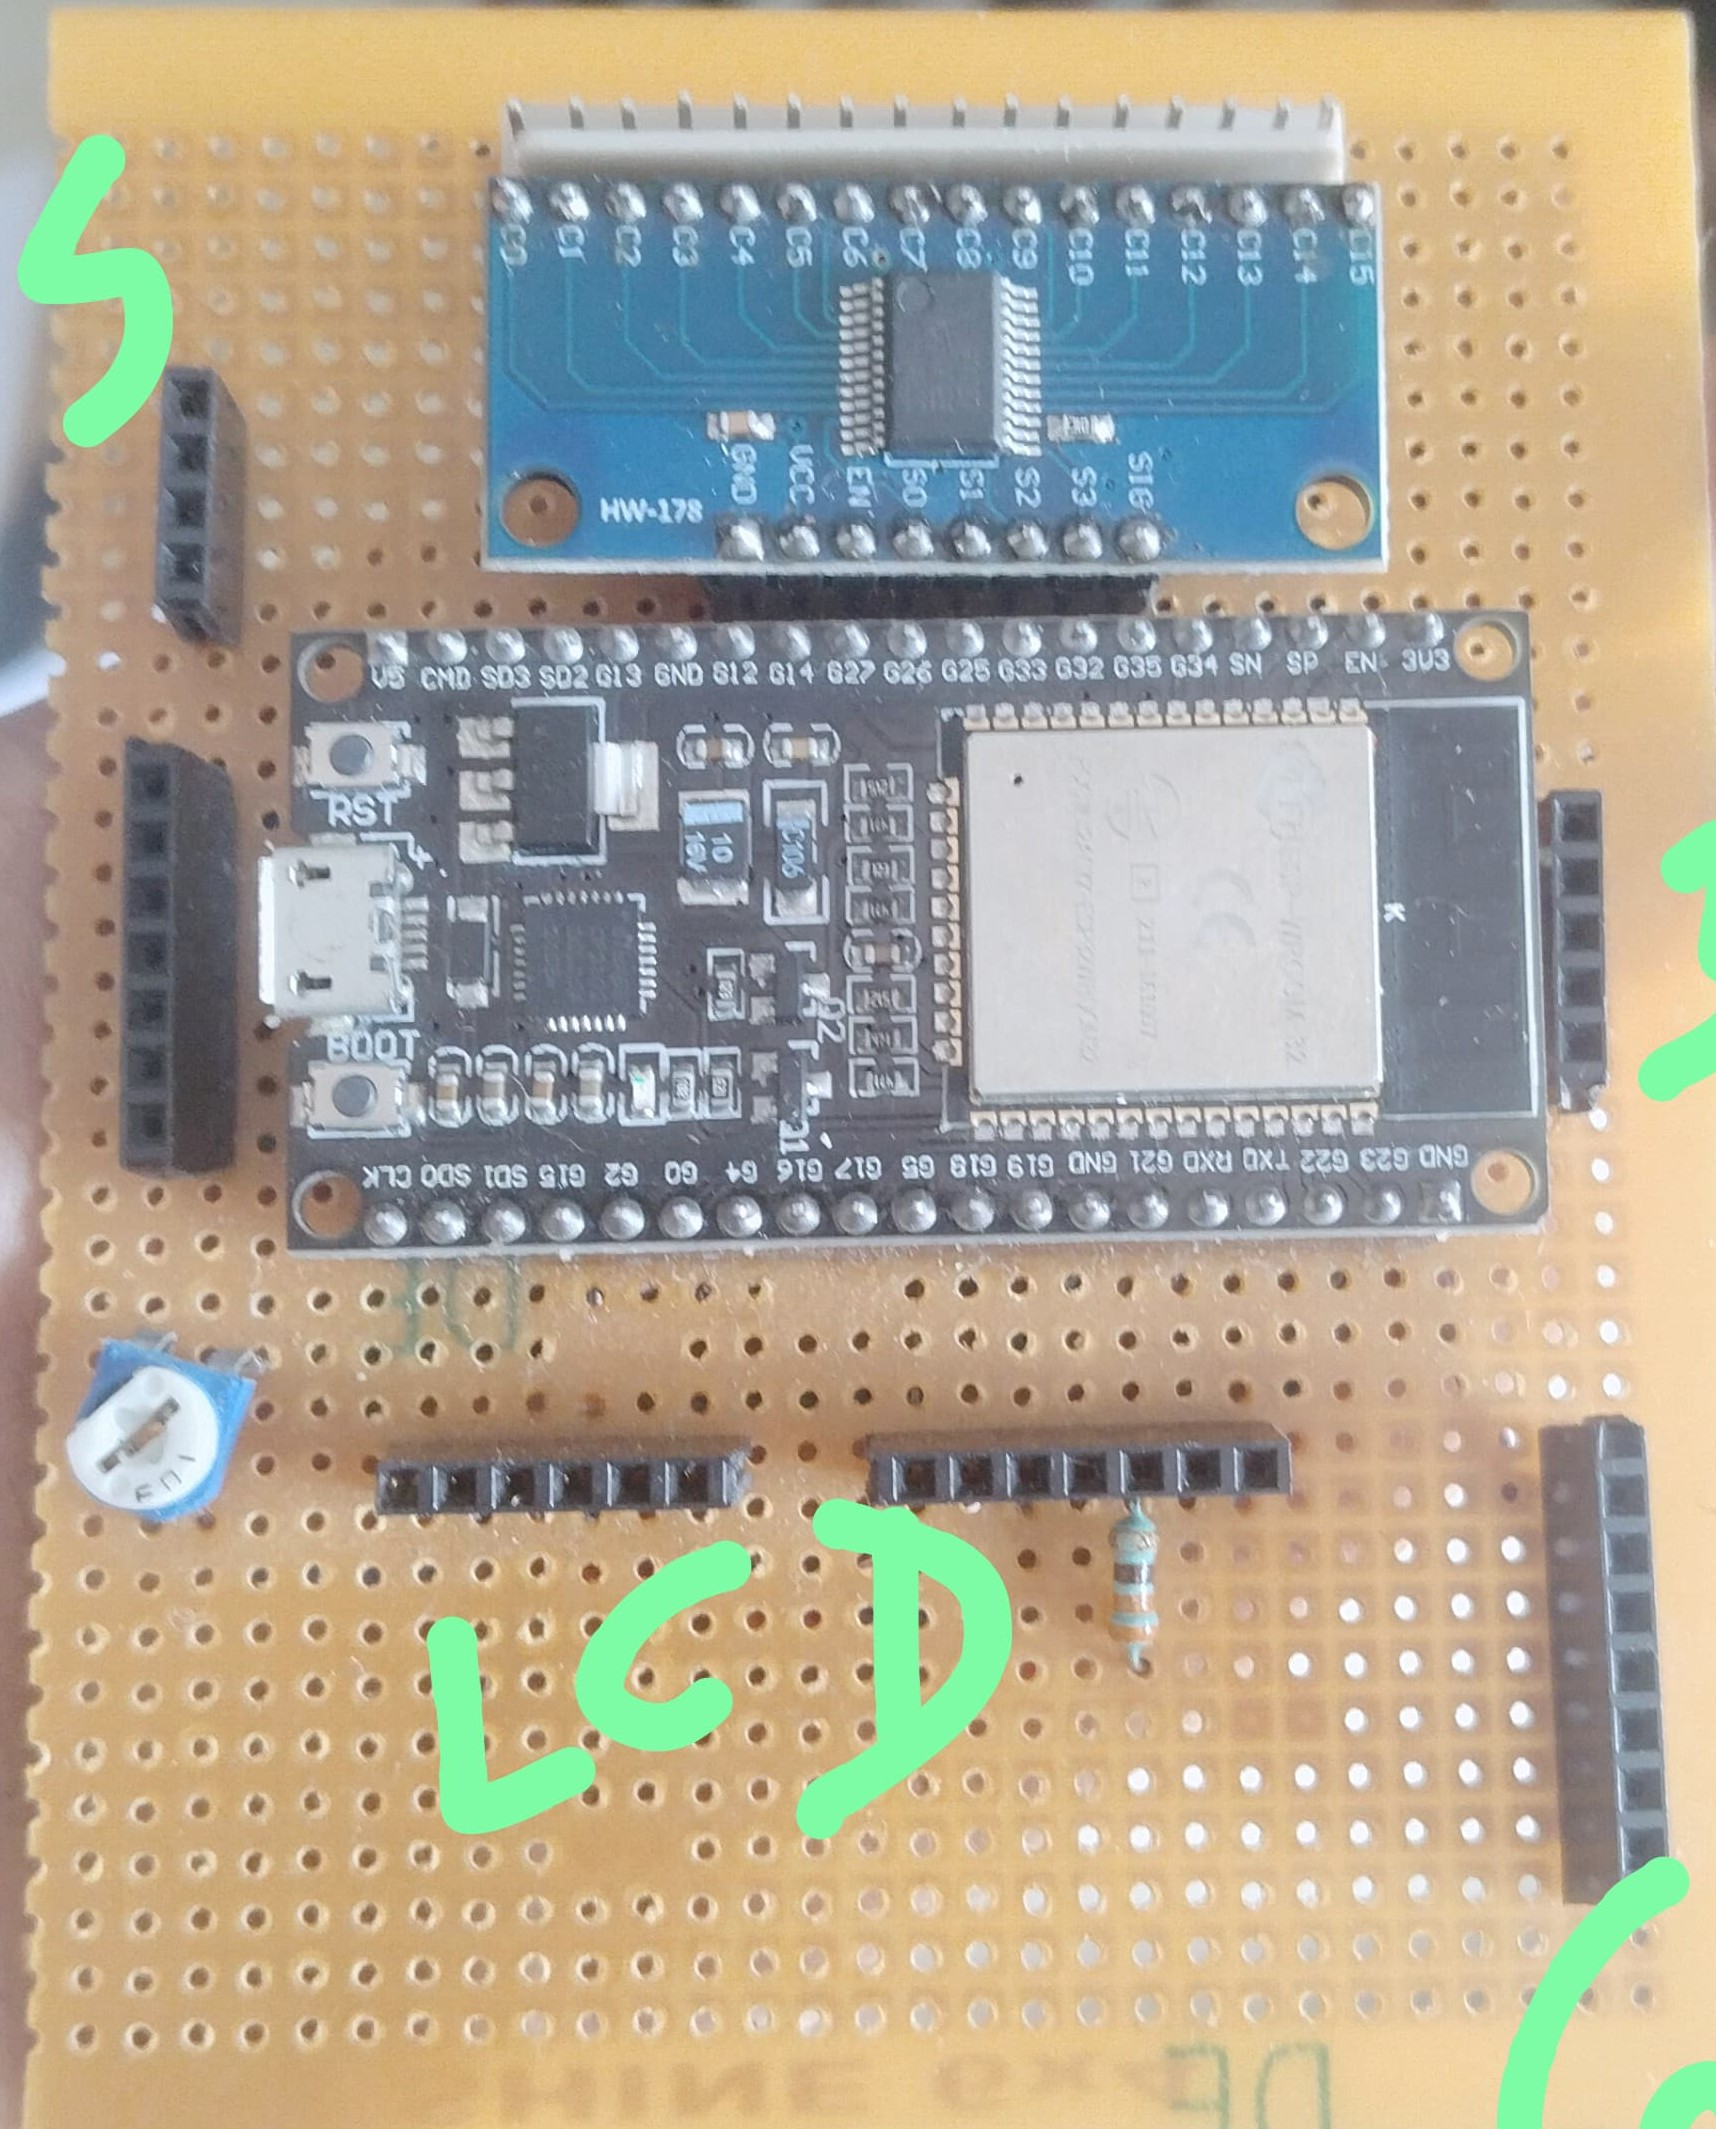
\includegraphics[width=\linewidth]{assets/pcb front.jpg}
        \caption{PCB (Front)}
        \label{fig:image1}
    \end{minipage}
    \hfill
    \begin{minipage}{0.47\textwidth}
        \centering
        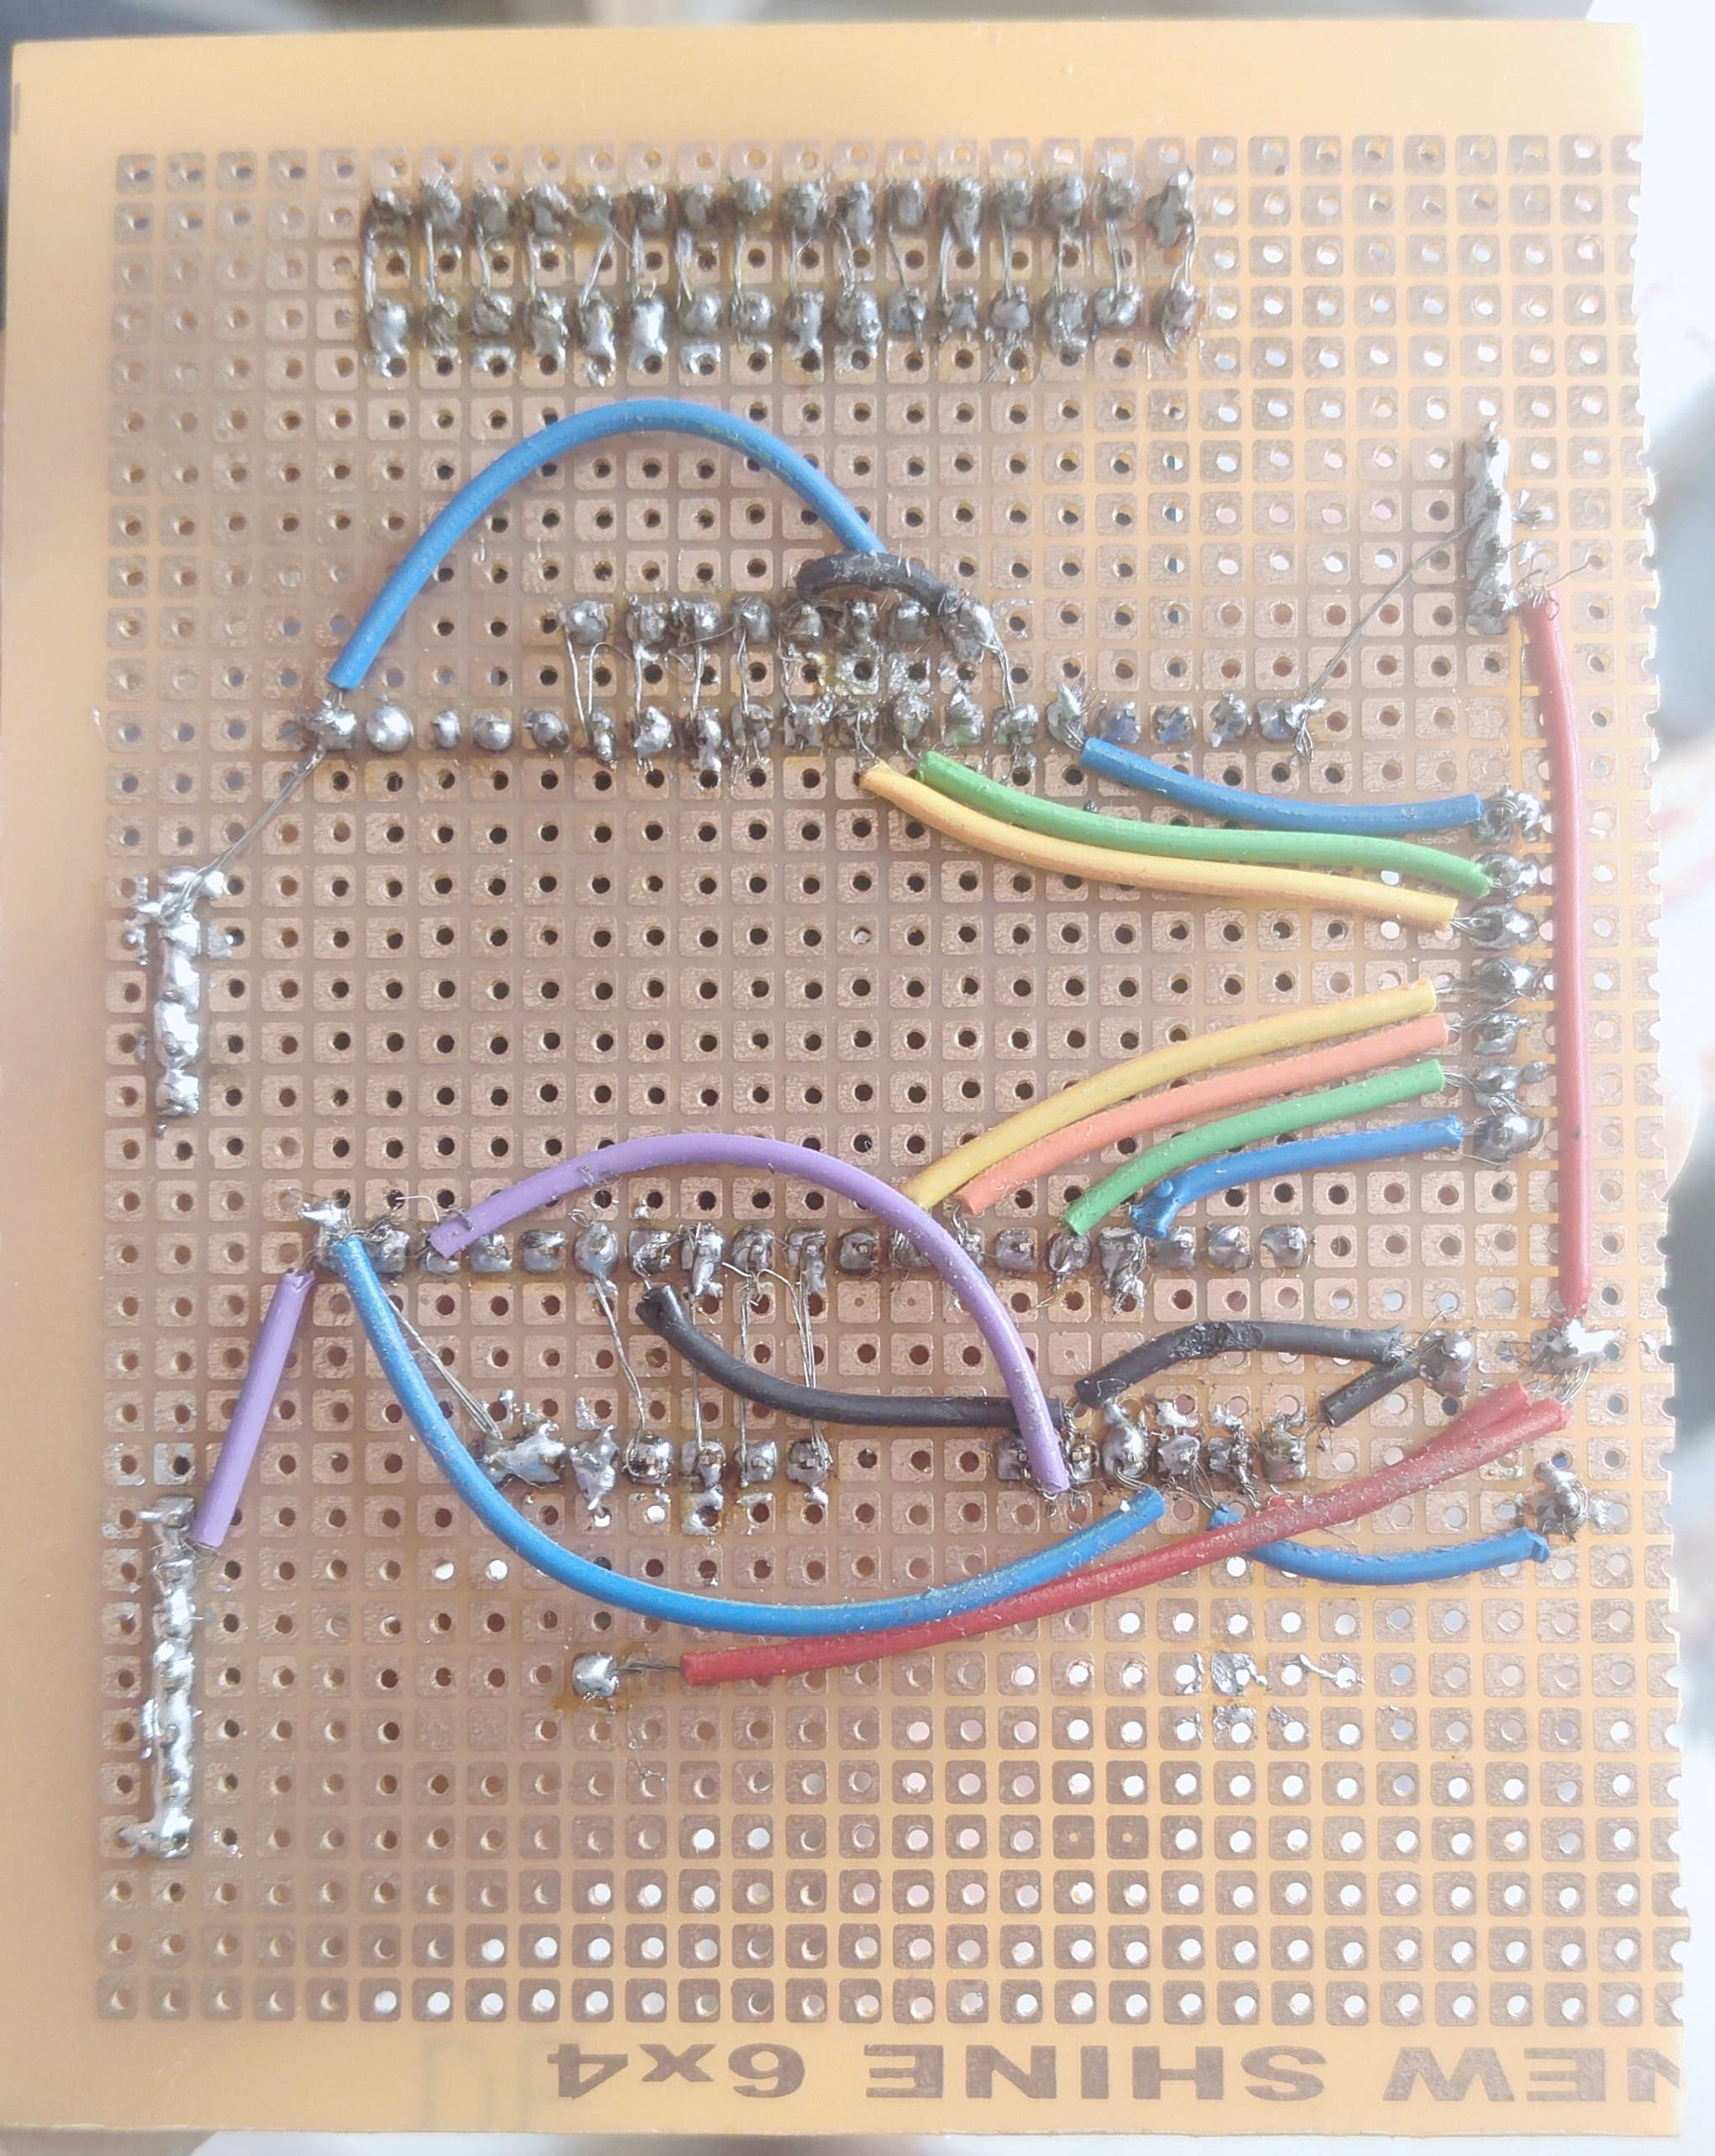
\includegraphics[width=\linewidth]{assets/pcb back.jpg}
        \caption{PCB (Back)}
        \label{fig:image2}
    \end{minipage}
\end{figure}

\begin{figure}
    \centering
    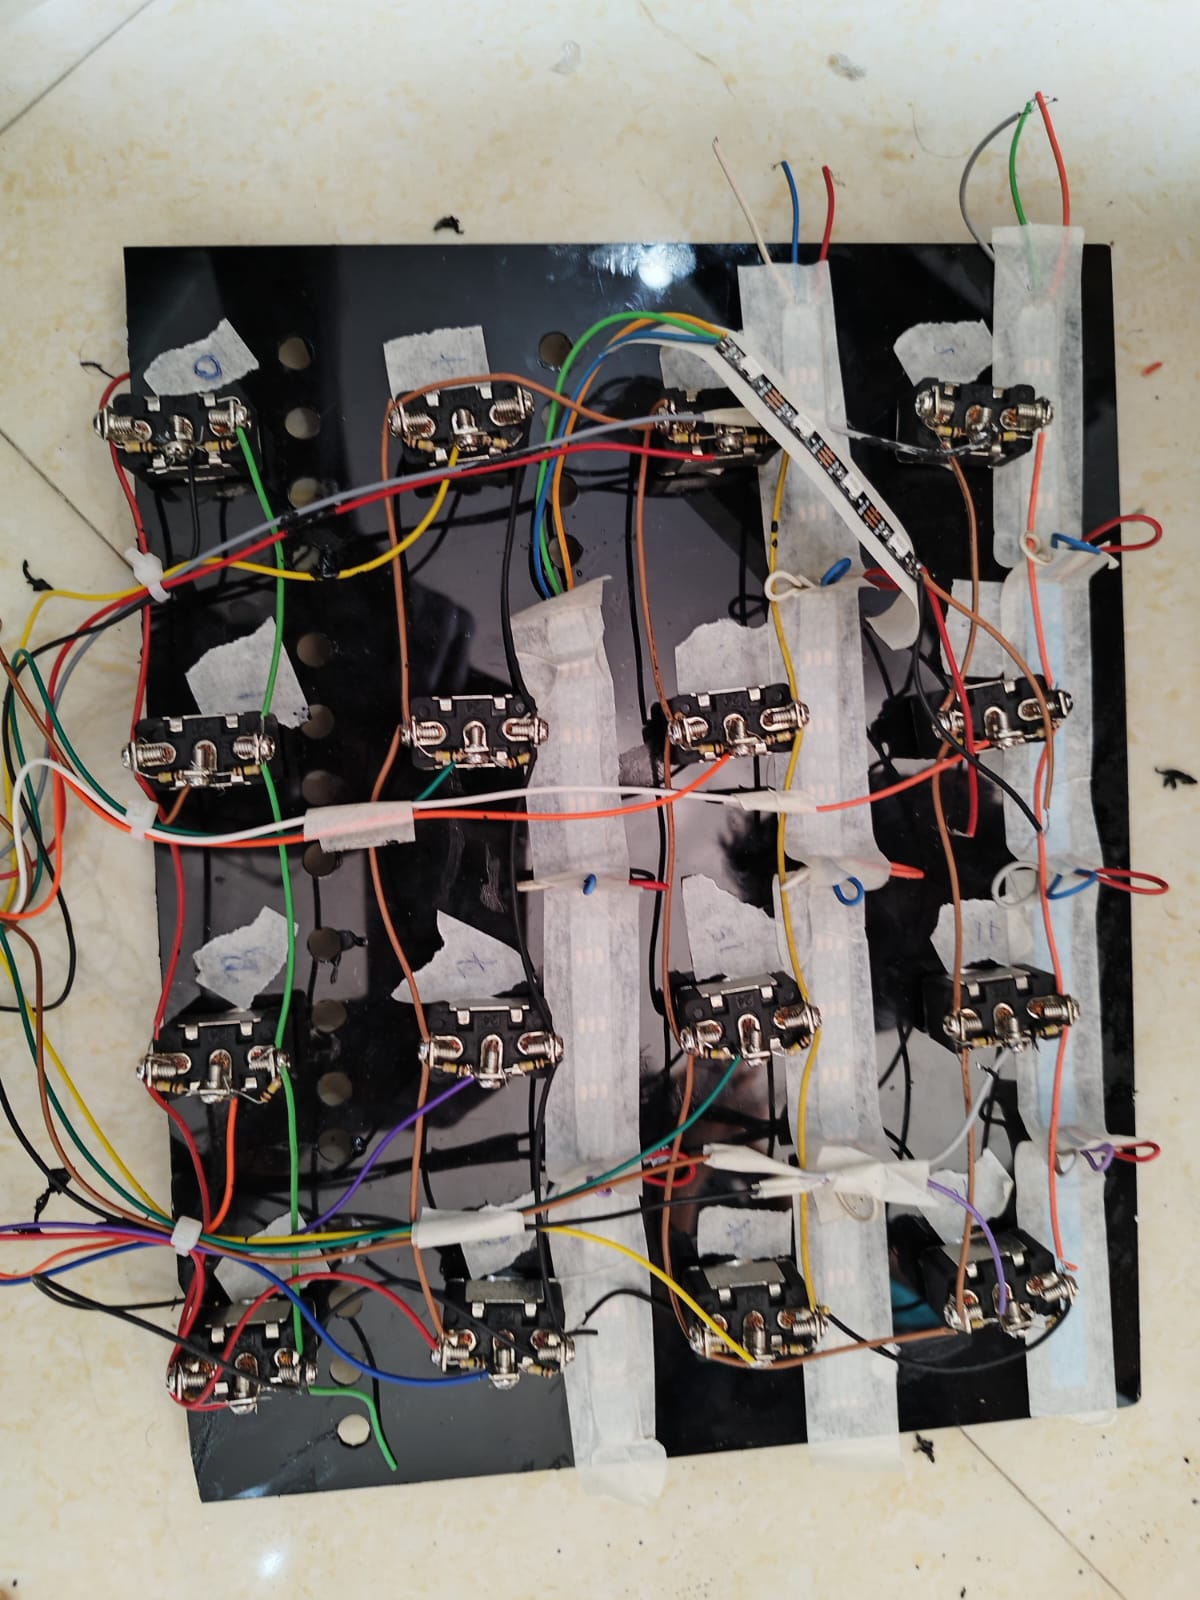
\includegraphics[angle=90,width=0.8\textwidth]{assets/switchboard.jpg}
    \caption{Switch board wiring}
    \label{fig:yourlabel}
\end{figure}

\newpage
\subsection{Enclosure Design}
The design was inspired from the Youtube video of channel “element14presents” on Arudino unit conversion calculator. Its design was modified to according to our needs.

\begin{figure}[h]
    \centering
    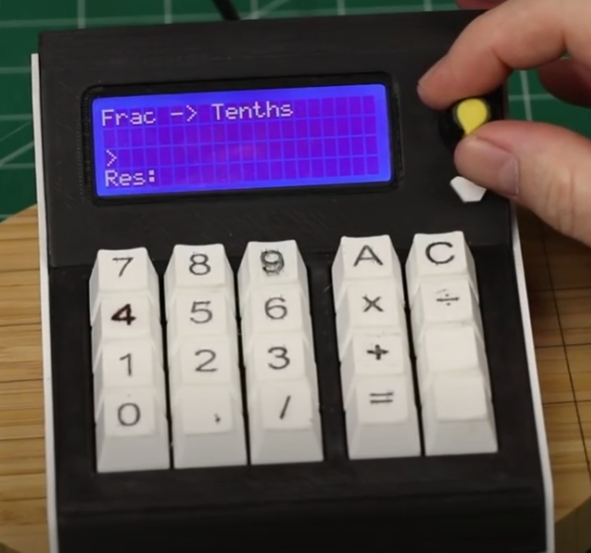
\includegraphics[width=0.3\textwidth]{assets/enclosure inspiration.png}
    \caption{Enclosure Inspiration}
    \label{fig:yourlabel}
\end{figure}
\begin{figure}[h]
    \centering
    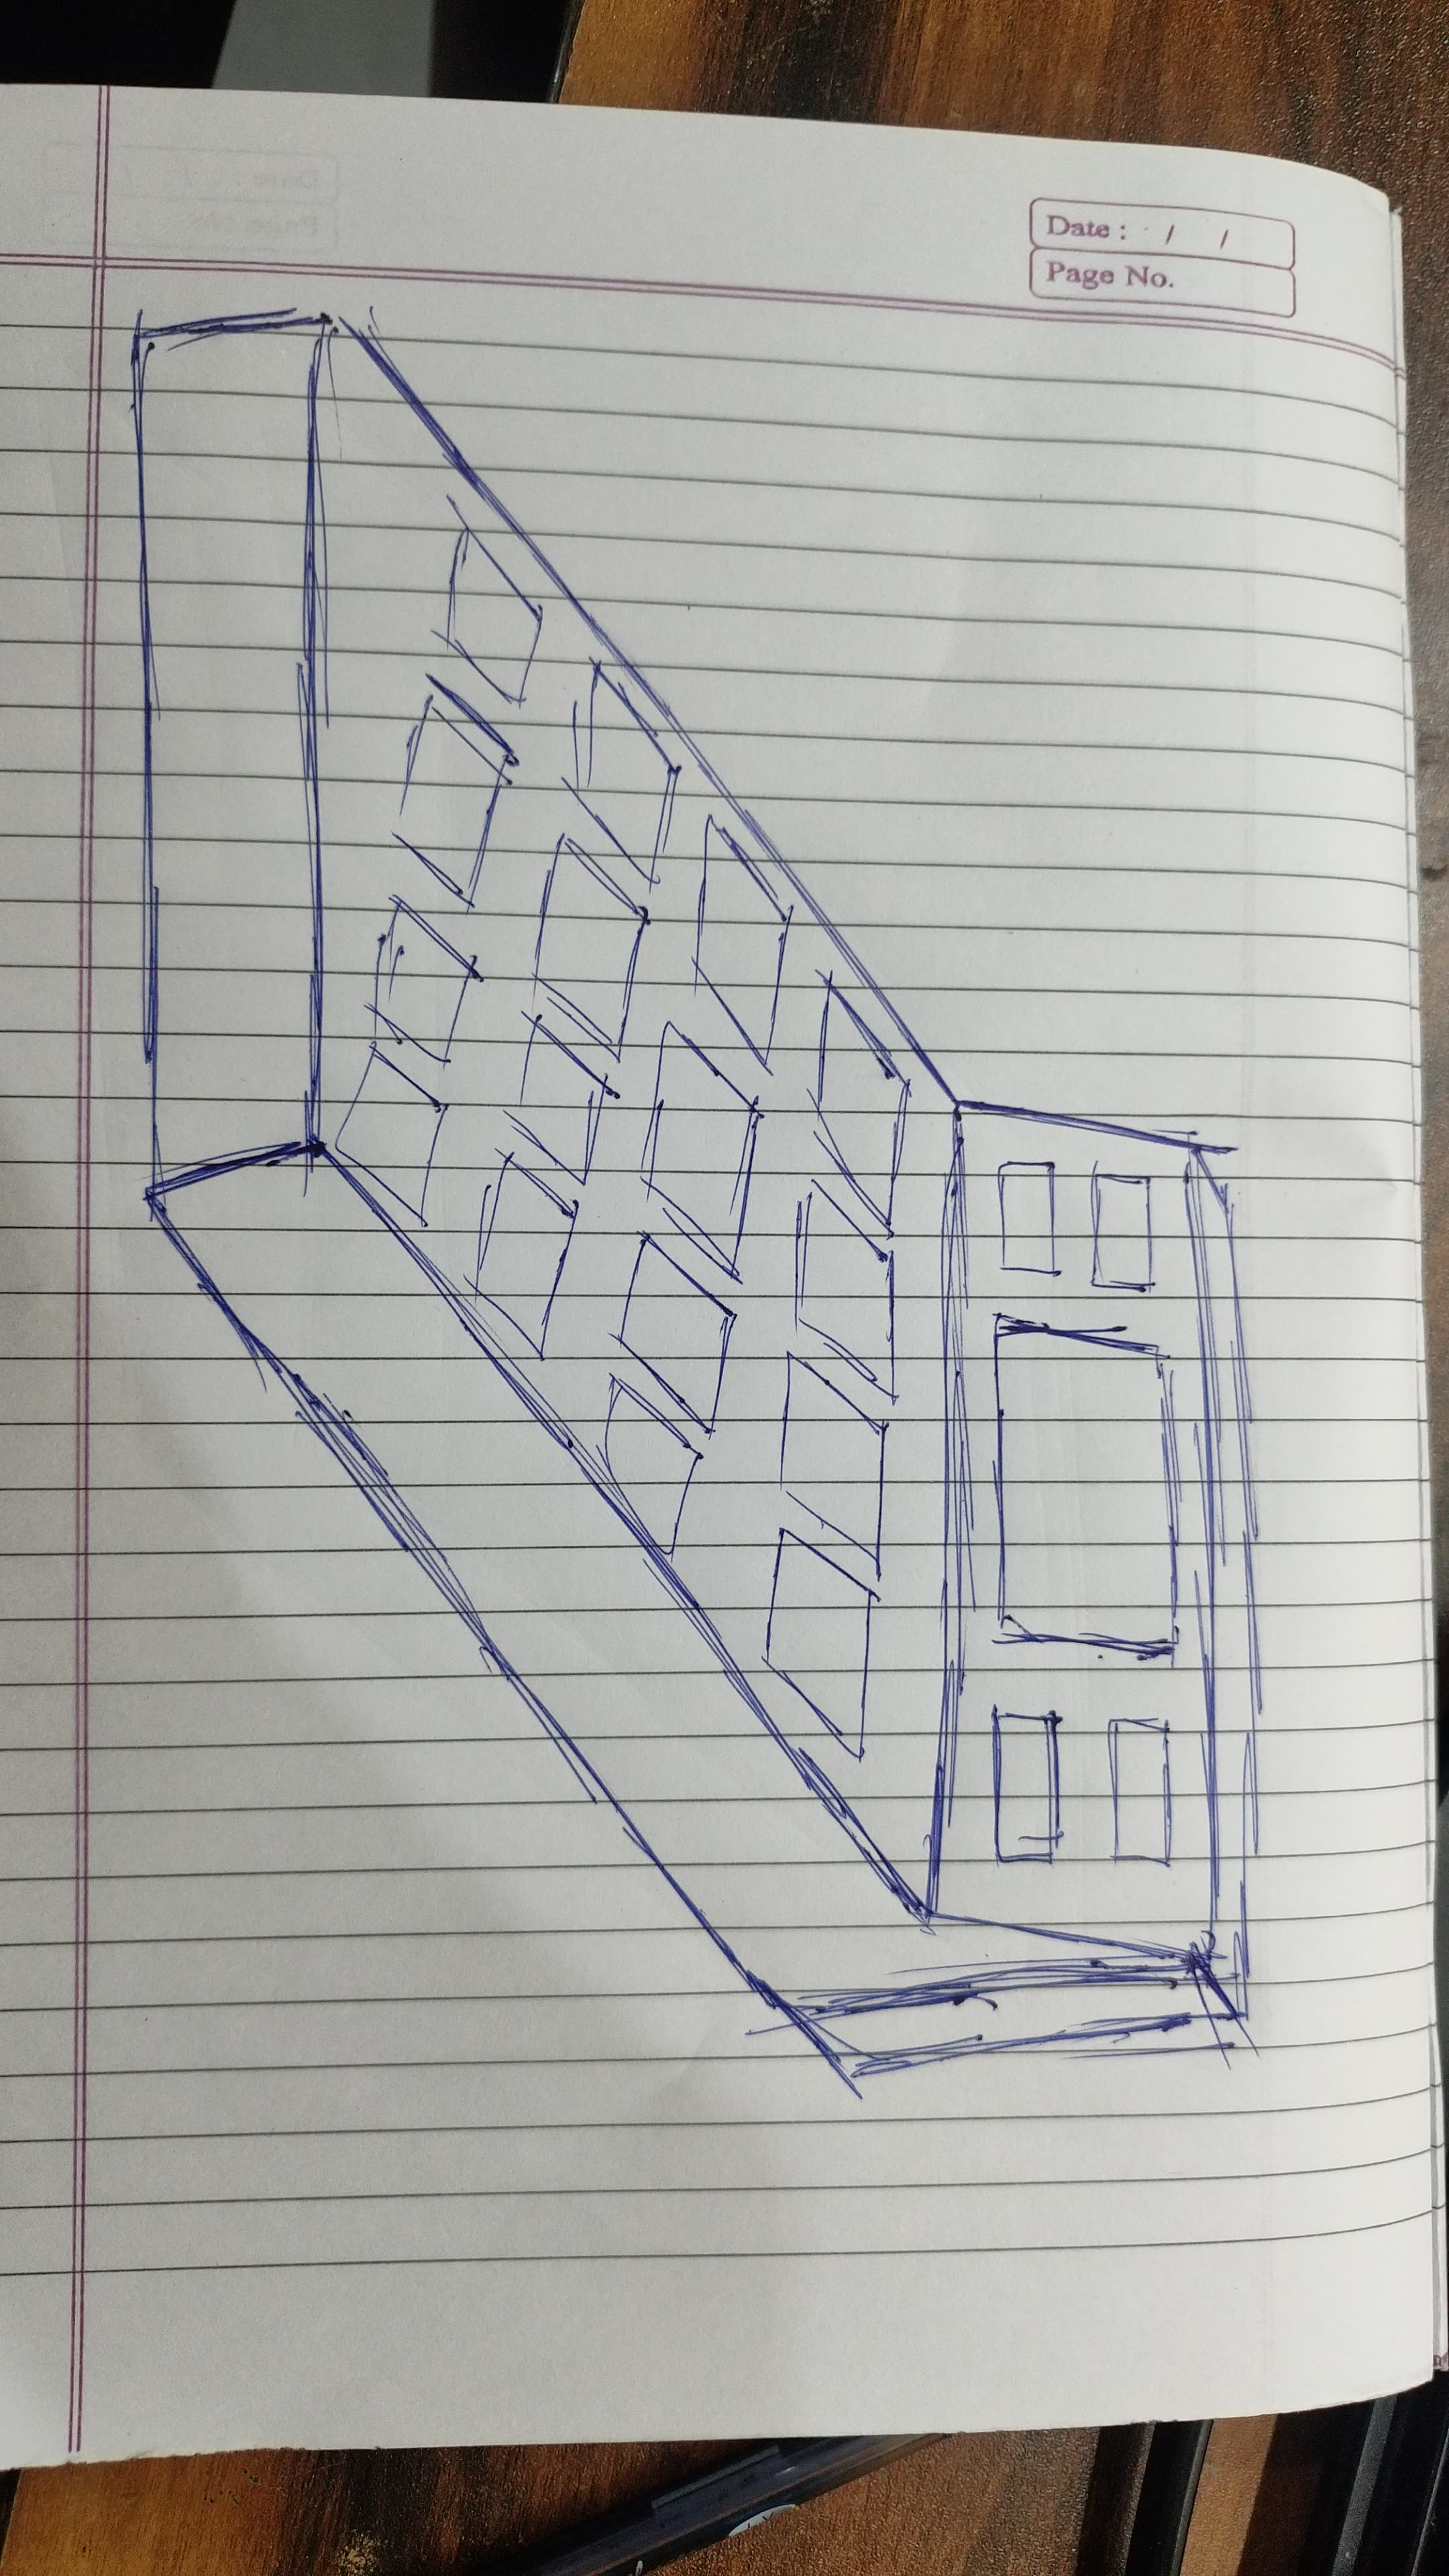
\includegraphics[angle=90,width=0.6\textwidth]{assets/rough sketch.jpg}
    \caption{Rough Sketch of Body}
    \label{fig:yourlabel}
\end{figure}
Enclosure was made using acrylic sheets. The dimensions for enclosure is around 25cm x 25cm. Each cell has dimensions of 6cm x 4cm. Drilling machine was used to make holes for switches ,LEDs etc. Glue gun was used to paste sheets with each other.
\begin{figure}[h]
    \centering
    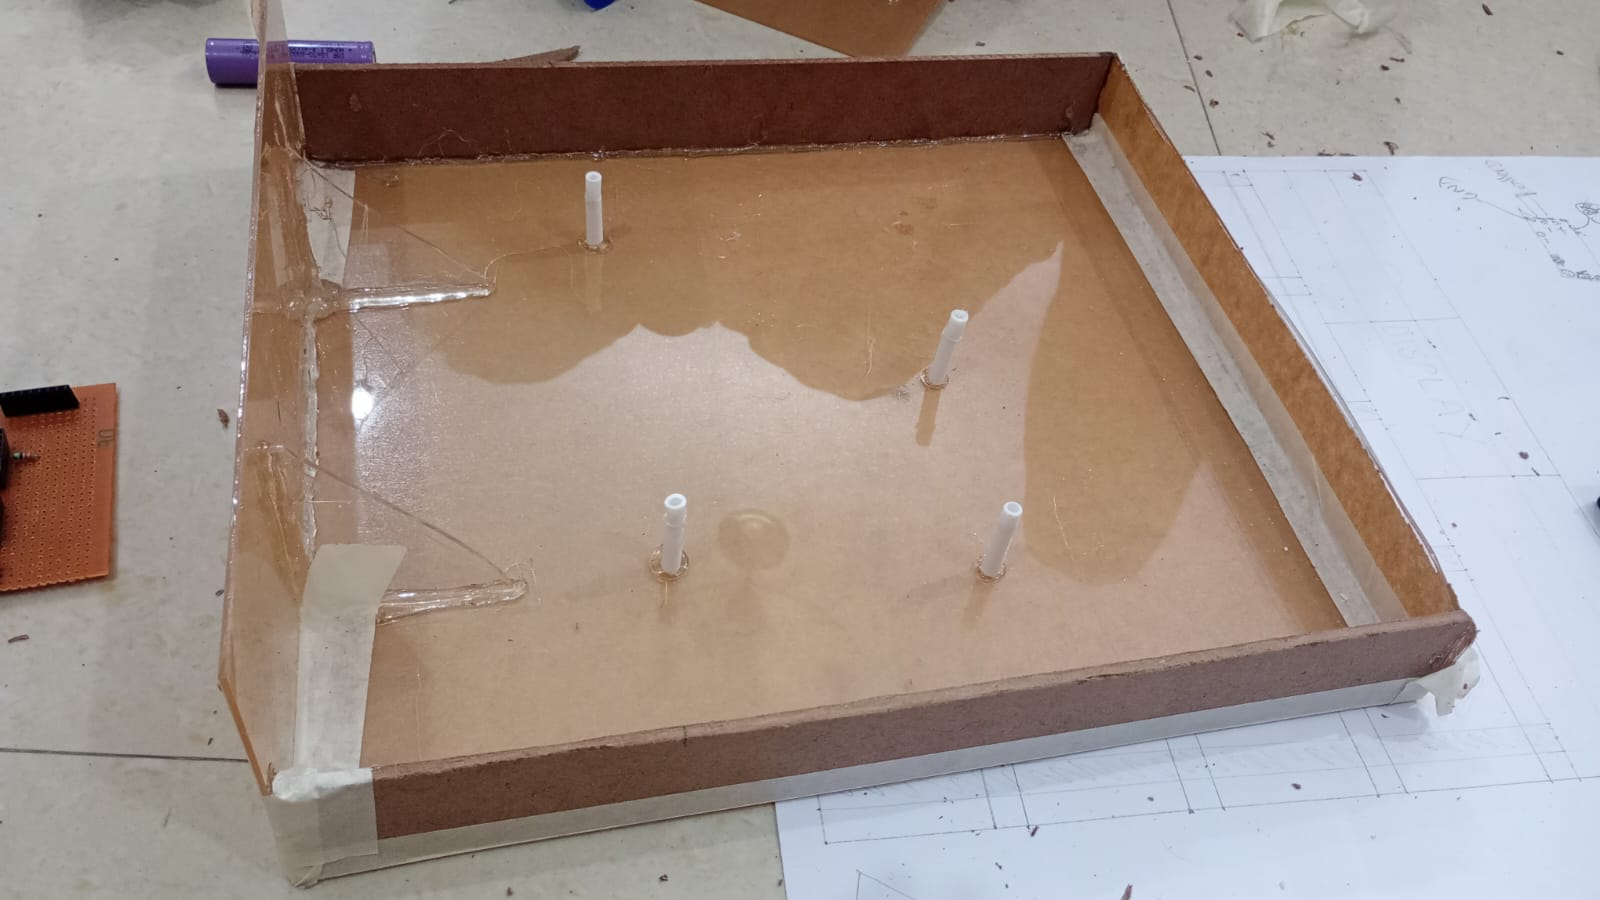
\includegraphics[width=0.7\textwidth]{assets/enclosure.jpg}
    \caption{Enclosure in Making}
    \label{fig:yourlabel}
\end{figure}

\newpage
\section{Software Overview}
The main language used is C++ in writing the code.Arudino IDE was used to write the ESP32 code. The software consists of mainly 3 files –
\begin{itemize}
    \item Custom K-Map library having .cpp extension
    \item K-Map library header file having .h extension
    \item ESP 32 Code file having .ino extension
\end{itemize}
The source code for the project is available on Github – \\
\url{https://github.com/alllhappy/K-Map-Calculator}
\subsection{Custom K-Map library (kmap.cpp)}
To solve the K-Map , we need to figure out groups of minterms. Then convert these minterms to their corresponding Boolean expression. Groups were identified using Quine–McCluskey algorithm(Tabulation method).This algorithm was used to make the  prime implicants chart.
Petrick Method was used to determine minimum groups required for a complete solution from this prime implicant chart.Both algorithms were hard coded specifically for the case of 4 variables .Final output will be of form \texttt{vector\textless vector\textless vector\textless int\textgreater \textgreater \textgreater \textgreater} containing all the possible solutions. This output will converted to 
\texttt{vector\textless string\textgreater}
 for the string solution.
\begin{verbatim}
{
    {{Grp1},{Grp2},...} ----> solution 1
    {{Grp1},{Grp2},...} ----> solution 2
    {{Grp1},{Grp2},...} ----> solution 3
}
\end{verbatim}
Above is the structure of final output(\texttt{vector\textless vector\textless vector\textless int\textgreater \textgreater \textgreater \textgreater})\\
The code is written using functional programming principles. 
\begin{figure}[h]
    \centering
    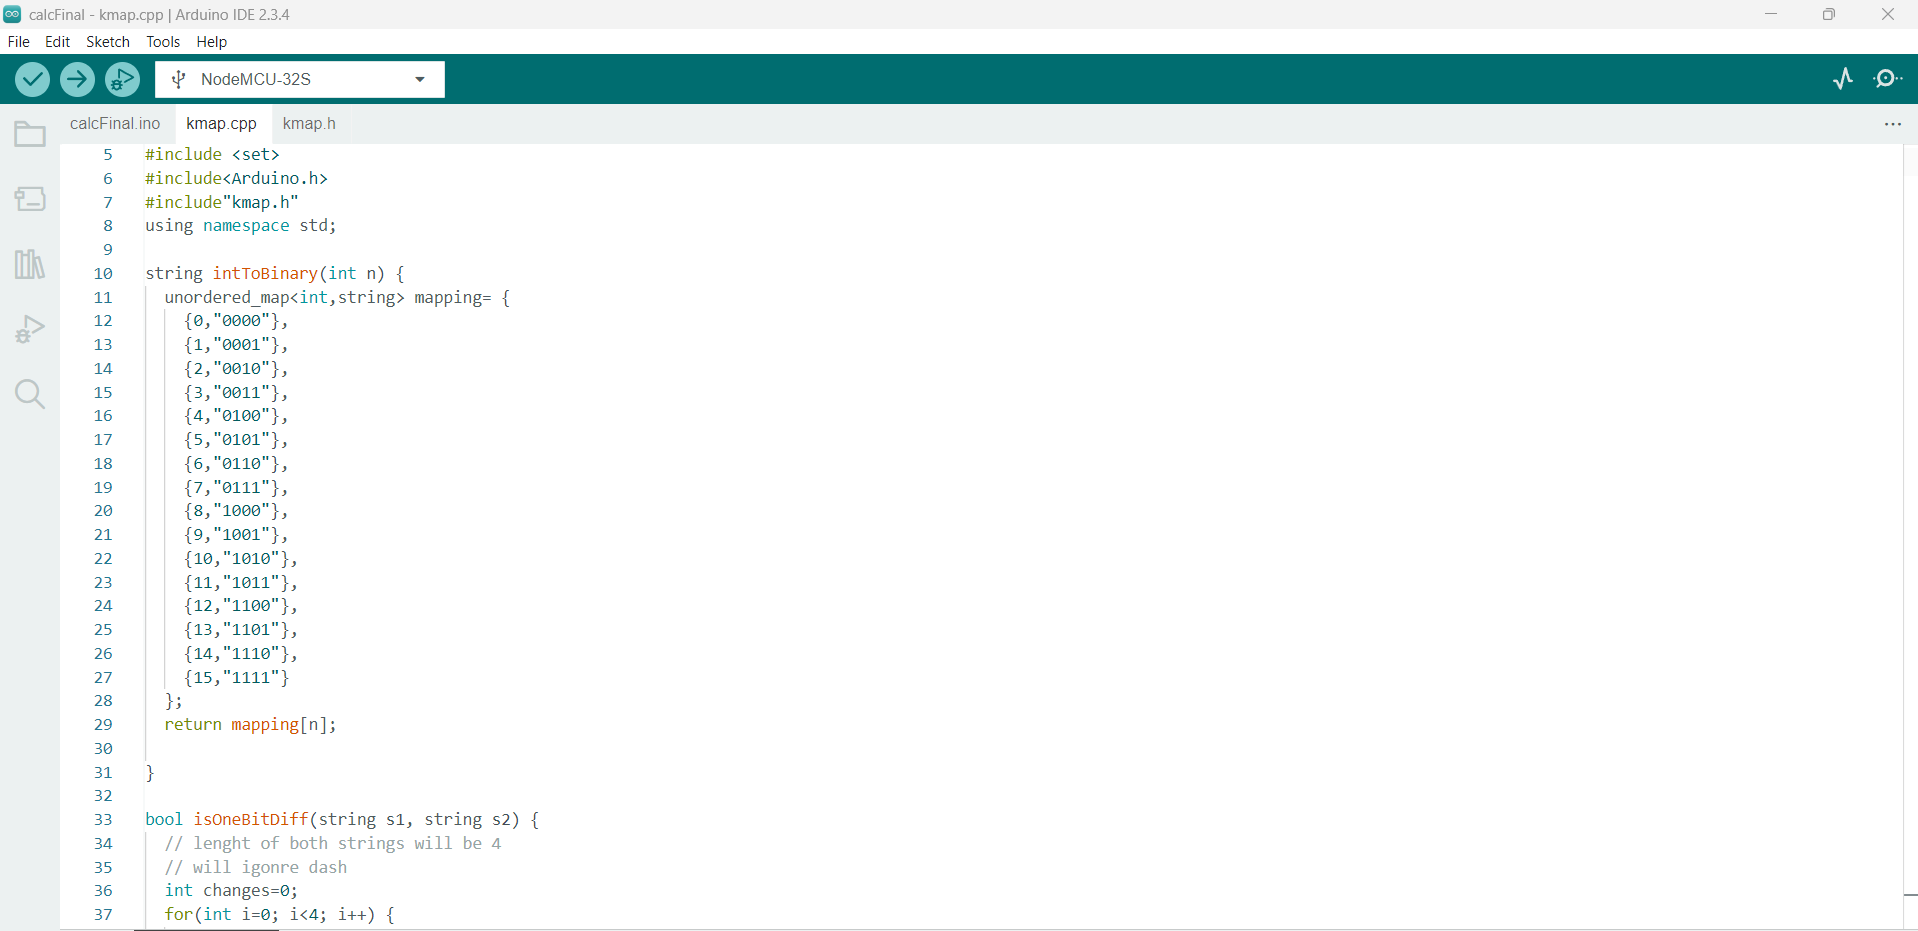
\includegraphics[height=0.35\textwidth]{assets/kmap code.png}
    \caption{Glimpse of kmap.cpp (entire file $\approx$ 900 lines)}
    \label{fig:yourlabel}
\end{figure}

\newpage
\subsection{K-Map library header file (kmap.h)}
\begin{figure}[h]
    \centering
    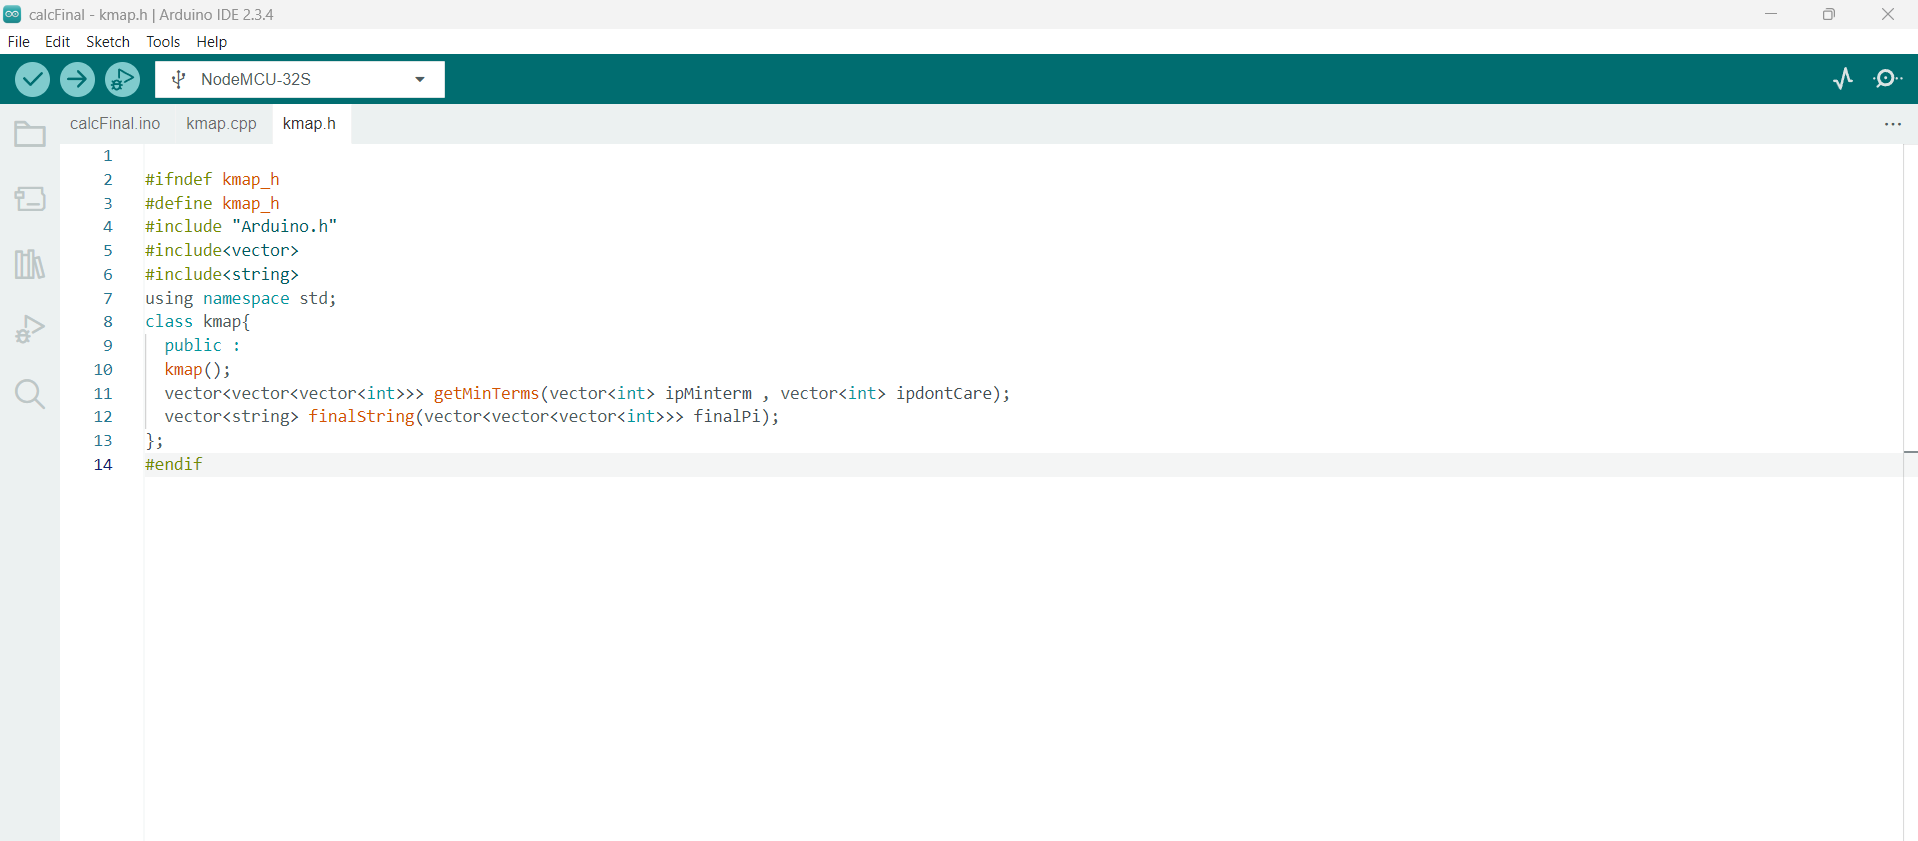
\includegraphics[height=0.35\textwidth]{assets/header file.png}
    \caption{kmap.h (entire file 14 lines) }
    \label{fig:yourlabel}
\end{figure}
This file is necessary  to import functions from the Kmap.cpp to ESP32 code, therefore existing as a bridge.
It exports only final 2 functions from Kmap.cpp which give final results.

\subsection{ESP32 code (calcFinal.ino)}
External libraries used in this code are –
\begin{itemize}
    \item LiquidCrystal – To control the display
    \item FastLED –  To control LED strips
    \item Kmap – To perform main Kmap logic
\end{itemize}
\begin{figure}[h]
    \centering
    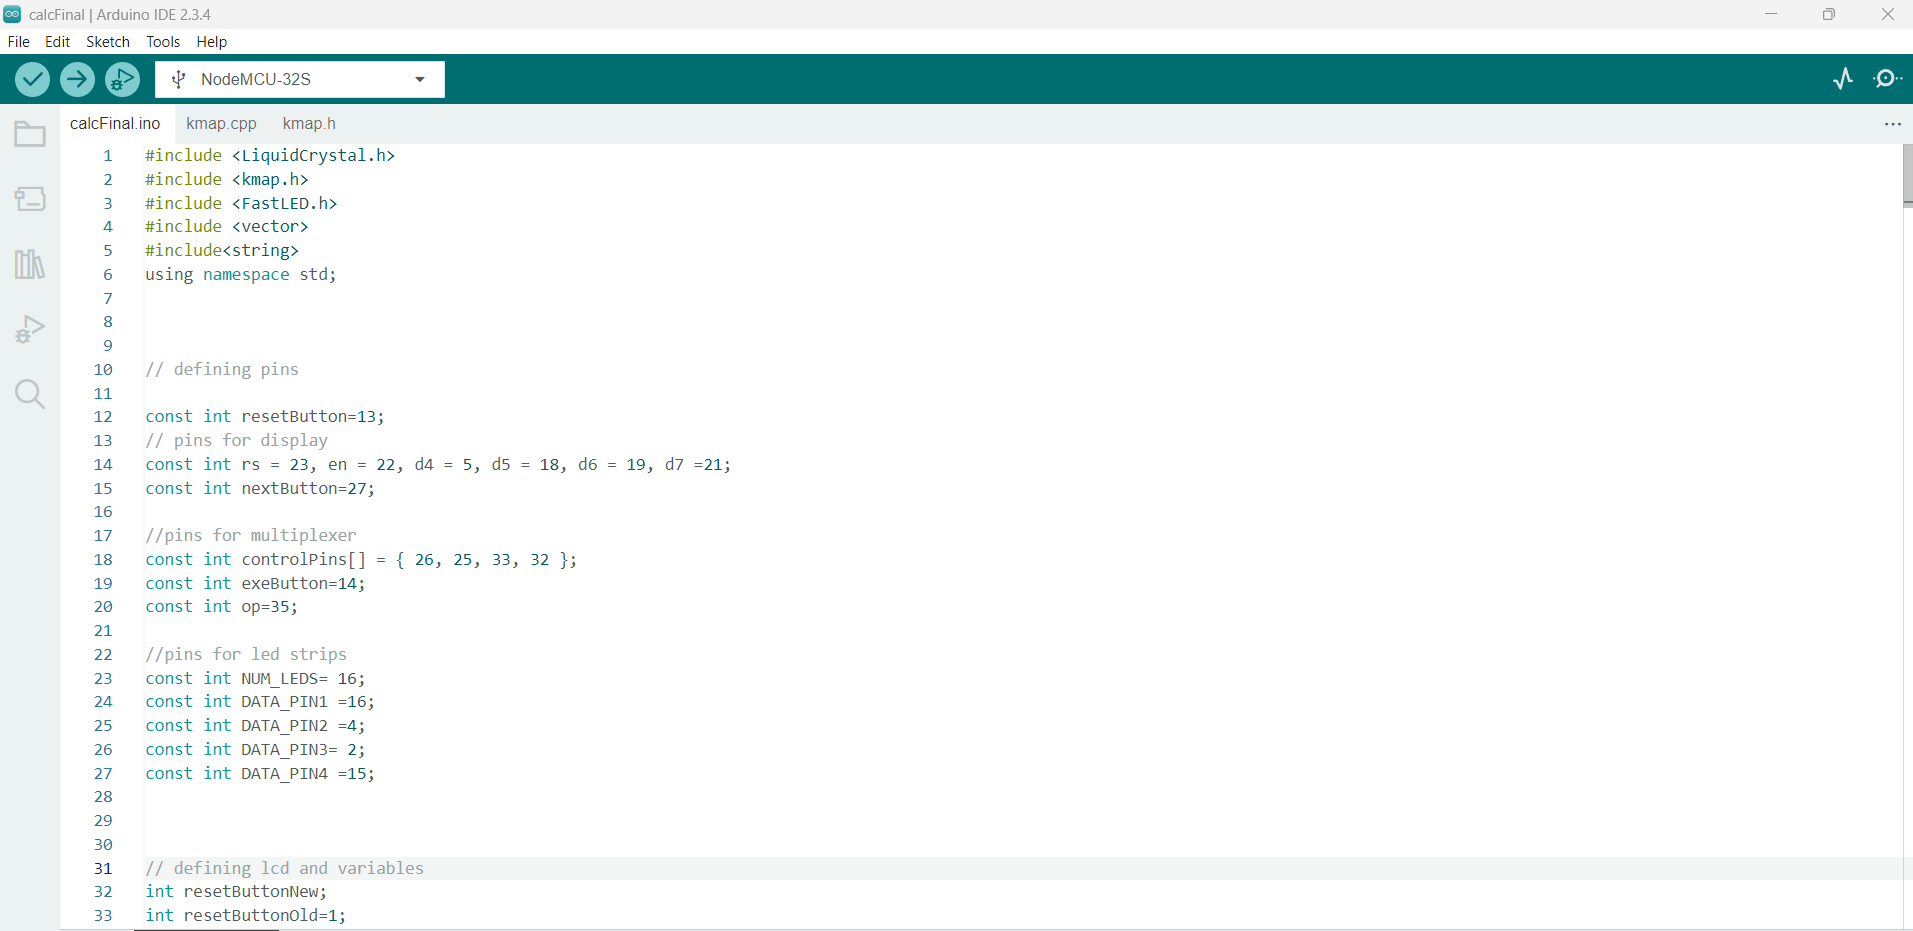
\includegraphics[height=0.35\textwidth]{assets/esp32 code.png}
    \caption{Glimpse of ESP32 code (entire file $\approx$ 400 lines)}
    \label{fig:yourlabel}
\end{figure}
When the calculator is turned on void setup() will run. It will initiate all the requirements. Also it will display a pattern of LEDs and display our names on LCD. After that everything will become. When the execute button is pressed the , ESP reads each channel of multiplexer one by one using analogRead() function. Using this this analog read values , each value is mapped to 0 ,1,2,3. (3 when analog Read is exactly 4095). 0 mapping represent logic don’t care. 1 represents logic 0 . 2\&3 represents logic 1. For example when switch is at middle so it will supply 1.5V to channel. analogRead() will give value around 2000 which is mapped to 1 which represents logic 0. This input is sent to two functions imported from kmap.cpp to perform necessary computations.
\\ \\
For setting the LEDs in the required pattern , each strip is set individually on the basis of the groupings given after the computation. For example if a  group is \{4,5\}  then cell 4 is present in 2nd strip therefore 2nd strip will be selected. It will check the 1st LED of cell 4. If it is on will move to the 2nd  LED of cell 4 otherwise it will light up the 1st LED with a color. For example let it be red. Now the 2nd cell in the same group is 5, It also comes in strip 2 , therefore it will be selected. Same process will repeat for cell 5. If more groups exist then same process will take place only the color will be changed. This is for first solution. If more solutions exist it will traverse to the solution 2 in output vector and set the output according to it.

\newpage
\section{Reflection}
\subsection{Problems Faced}
\textbf{Choosing Wrong Pins of ESP32}\\
Used that pins of ESP32 for GPIO purposes which are not recommended. For example initially a push button was assigned pin SensorVP. The switch was at pressed condition even when it was not pressed. This was due to the reason that pin SensorVP do not have built in pull up or pull down resistor which was configured in code.\\
\textit{Solution : Pins for push buttons were changed}\\

\textbf{Use of Unreliable Wires}\\
Initially all the wirings and PCB were made using very thin wires which broke easily. This led to  an unreliable system. Sometimes wires shorted in PCB. Sometimes wires broke or became loose from switches \& LEDs. \\
\textit{Solution : PCB was made again using reliable single core wires. All weak wiring was replaced by strong wires.}\\

\textbf{Boost Power Failure }\\
In starting our plan was to boost the 3.7V supply using a XL6009 step up to provide a constant 5V output. However when the circuit was physically realized and tested , even after setting the voltage to 5V for output in booster it supplied a 26V spike to the ESP32 and LEDs . Since no protection circuit was implemented it shorted the LED’s. Although ESP32 was functional but it was not recognised by our laptops when connected via cable , therefore not able to upload any new code.\\
\textit{Solution : Took the step down approach. Got new ESP32 and LED strips.}
\subsection{Further Improvements}
This calculator specifically solves the case of 4 variable K-Map. Although it can be used to display groupings for case of 2,3 variables by using only appropriate cells, the string solution will be wrong in that case. This calculator could have an additional input about number of variables the user want to use and set the output accordingly. \\
Printed PCBs are of superior quality therefore can be used instead of using a zeroboard. Also a 3D printed enclosure will look more professional and aesthatic.
\subsection{Conclusion}
A calculator to solve a K-Map for 4 variables was physically realized. This calculator is exactly what we visioned at the start of the project. Estimated time to make whole project was about a month. Estimated cost was around  \rupee 2000 .
\newpage
\section{References}
\begin{enumerate}
    \item \url{https://en.wikipedia.org/wiki/Karnaugh_map}
    \item \url{https://en.wikipedia.org/wiki/Quine%E2%80%93McCluskey_algorithm}
    \item \url{https://en.wikipedia.org/wiki/Petrick%27s_method}
    \item \url{https://byjus.com/gate/various-implicants-in-k-map-notes/#:~:text=A%20group%20of%20squares%20or,are%20formed%20in%20K-Map.}
    \item \url{https://www.boolean-algebra.com/kmap/}
    \item \url{https://randomnerdtutorials.com/esp32-pinout-reference-gpios/}
    \item \url{https://youtu.be/LdpvCepML-E?si=mHEXBt-v1sGeoXkl}
    \item \url{https://youtu.be/wR1G2RamHj4?si=qs5A7fxIRTOI7eHX}
\end{enumerate}

\end{document}
